\documentclass[reprint,pre,aps]{revtex4-1}

\usepackage{amsmath}
\usepackage{amssymb}
\usepackage{graphicx}
\usepackage[hidelinks]{hyperref}

\renewcommand{\thesection}{\arabic{section}}
\renewcommand{\thesubsection}{\thesection.\arabic{subsection}}
\renewcommand{\thesubsubsection}{\thesubsection.\arabic{subsubsection}}

\makeatletter
\renewcommand{\p@subsection}{}
\renewcommand{\p@subsubsection}{}
\makeatother

\begin{document}

\title{NKN: a Scalable Self-Evolving and Self-Incentivized Decentralized Network}

\author{NKN Lab\\www.nkn.org}
\noaffiliation

\date{\today\ \ Version: 1.0}


\begin{abstract}
NKN (New Kind of Network) is a new generation of highly scalable, self-evolving and self-incentivized blockchain network infrastructure. NKN addresses the network decentralization and self-evolution by introducing Cellular Automata (CA) methodology \cite{wolfram1983statistical, wolfram2002new} for both dynamism and efficiency. NKN tokenizes network connectivity and data transmission capacity by a novel and useful Proof of Work. NKN focuses on decentralizing network resources, similar to how Bitcoin \cite{nakamoto2008bitcoin} and Ethereum \cite{buterin2014next} decentralize computing power as well as how IPFS \cite{benet2014ipfs} and Filecoin\cite{filecoin} decentralize storage. Together, they form the three pillars of the Internet infrastructure for next generation blockchain systems. NKN ultimately makes the network more decentralized, efficient, equalized, robust and secure, thus enabling healthier, safer, and more open Internet.
\end{abstract}

\maketitle

\onecolumngrid

\vspace{-0.2in}

\tableofcontents

\clearpage

\twocolumngrid

\section{Challenges}

After years of transmutation, the Internet is in danger of losing its original vision and spirit. For example, Network Neutrality is overturned \cite{restore_internet_freedom}; spectrum and bandwidth are not efficiently utilized; information is fragmented and can be censored; privacy protection is limited. These signal that the network needs a reform.

Existing solutions are not suitable for next generation blockchain systems due to the following reasons:
\begin{itemize}
\item Utilize a centralized approach to improve efficiency.
\item Sacrifice the scalability of the network to speed up consensus.
\item Limit participation rate of nodes or require authorization to increase ``security''.
\item Use purely financial motivations or trusted third parties to solve problems which should be solved by mathematics and technology.
\end{itemize}

\subsection{Limitations of P2P Networks}

Peer-to-peer (P2P) networks currently face several major challenges, which are the opportunities for NKN.  First static network topology is vulnerable to faulty and malicious attack. Second, there is no economic self-incentivized scheme for network connectivity and data transmission. Finally, network scalability is widely sacrificed to enhance controllability. These are all to be solved by the NKN as shown in Fig.~\ref{fig:feature_compare}.

\begin{figure}[!htp]
\centering
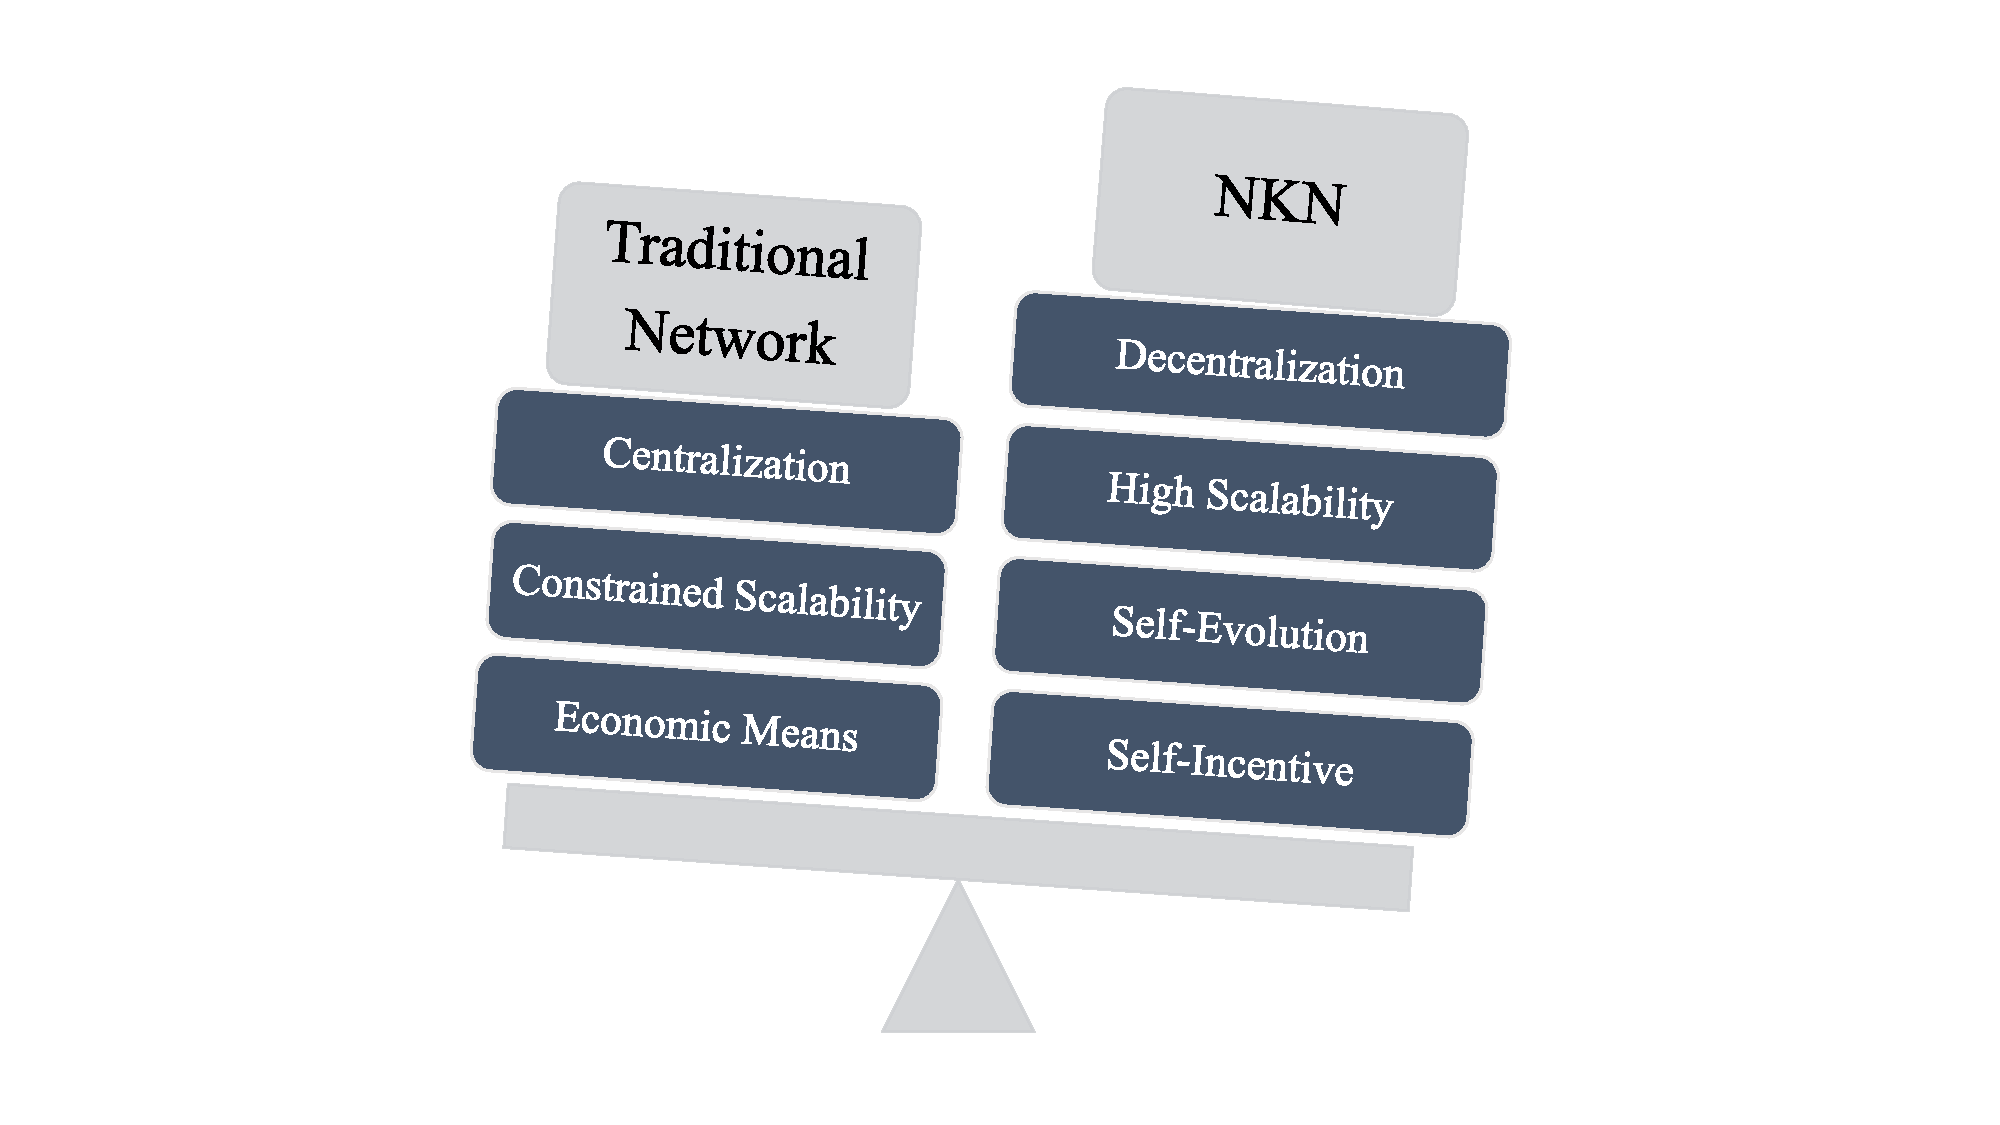
\includegraphics[width=0.8\linewidth]{fig/feature_compare}
\caption{Feature comparisons between existing solutions and NKN.}
\label{fig:feature_compare}
\end{figure}

\subsection{Resource Utilization}

A highly reliable, secure and diverse Internet is essential to everyone. Yet, huge inefficiency exists in the current network when providing global connectivity and information transmission. It's time to rebuild the network we want, not just patch the network we have. A fully decentralized and anonymous peer-to-peer system offers huge potential in terms of improved efficiency, sustainability and safety for industry and society.

\subsection{Net Neutrality \& Fragmentation}

When the Federal Communications Commission (FCC) approved a measure to remove the net neutrality rules by the end of 2017 \cite{restore_internet_freedom}, a demand of ending our reliance on big telecommunication monopolies and building decentralized, affordable, locally owned Internet infrastructure becomes ever stronger. The unrestricted and private Internet access environment is becoming unsustainable under an endless stream of attacks and blockage, leading to selective and biased information propagation. Without a proper incentivizing engagement scheme, it is almost impossible to maintain a constant and secured information propagation channel.

Furthermore, Internet has become fragmented due to various reasons. This not only exacerbates separation but also negatively impacts innovation of science, technology and economy.

\section{Vision}

NKN intends to revolutionize the entire network technology and business. NKN wants to be the Uber or Airbnb of the trillion-dollar communication service business, but without a central entity. NKN aspires to “free the bits, and build the Internet we always wanted”.

\subsection{Objectives of NKN}

NKN sets the following objectives:

\begin{itemize}
\item Any node can connect to this fully open network from any place
\item Promote network sharing
\item Secure net neutrality from network layer innovations
\item Always keep network open and scalable
\item Perform efficient and dynamic routing
\item Tokenize network connectivity and data transmission assets and incentivize participating nodes
\item Design and build the next generation of blockchain network
\end{itemize}

\subsection{The Third Pillar: Networking}

By blockchainizing the third and probably the last pillar of Internet infrastructure, NKN will revolutionize  the blockchain ecosystem by innovating on the network layer, after Bitcoin \cite{nakamoto2008bitcoin} and Ethereum \cite{buterin2014next} blockchainized computing power as well as IPFS \cite{benet2014ipfs} and Filecoin\cite{filecoin} blockchainized storage. The next generation blockchains based on NKN are capable of supporting new kind of decentralized applications (DApp) which have much more powerful connectivity and transmission capability. The vision of NKN is not only to revolutionize the decentralized network layers, but also to develop core technologies for the next generation blockchain.

\begin{figure}[!htp]
\centering
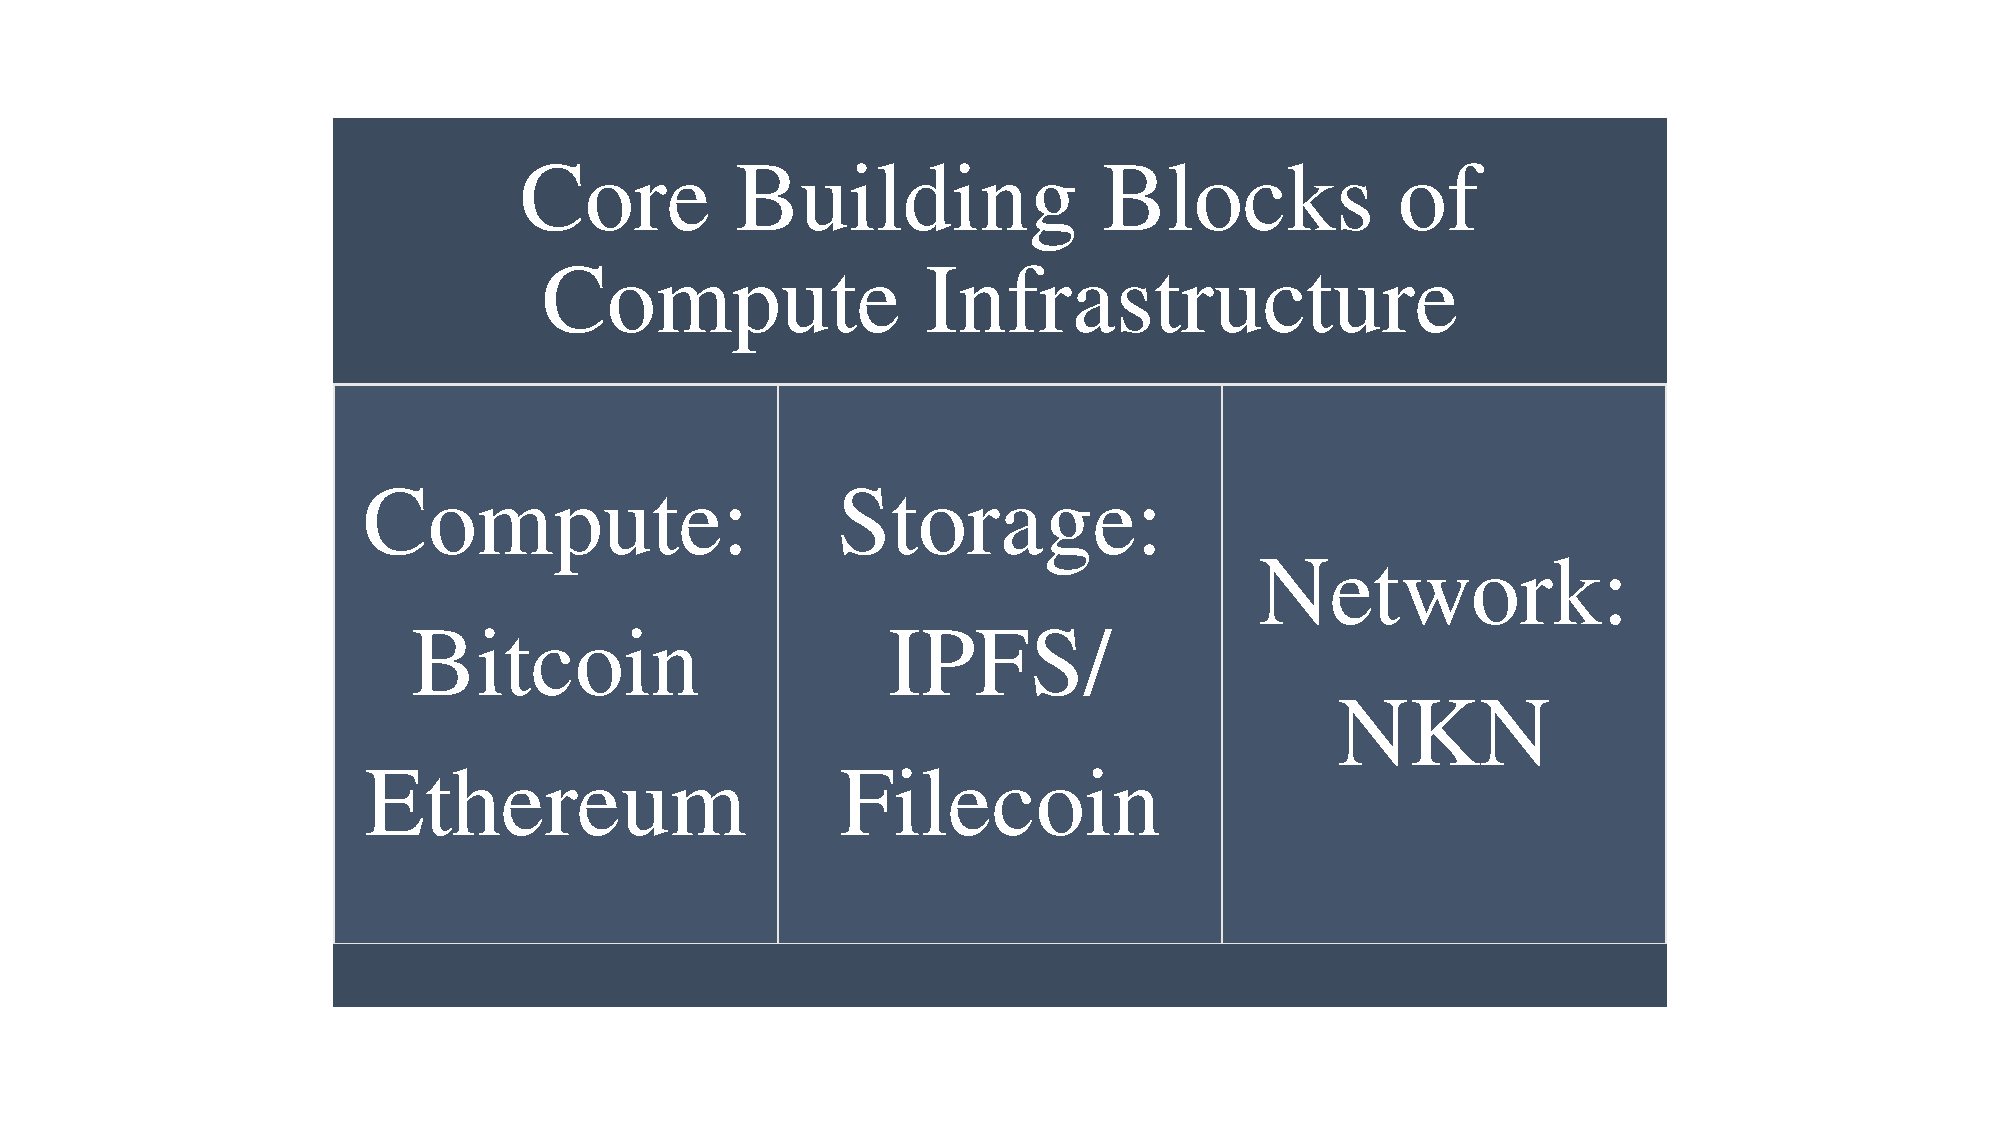
\includegraphics[width=0.6\linewidth]{fig/core_blocks_compute_infra}
\caption{NKN as the 3rd pillar of blockchainized Internet infrastructure.}
\label{fig:core_blocks_compute_infra}
\end{figure}

\subsection{Elementary Components}

NKN builds upon several innovative elementary components that are different from existing solutions, as shown in Fig.~\ref{fig:elementary_components}.

\begin{figure}[!htp]
\centering
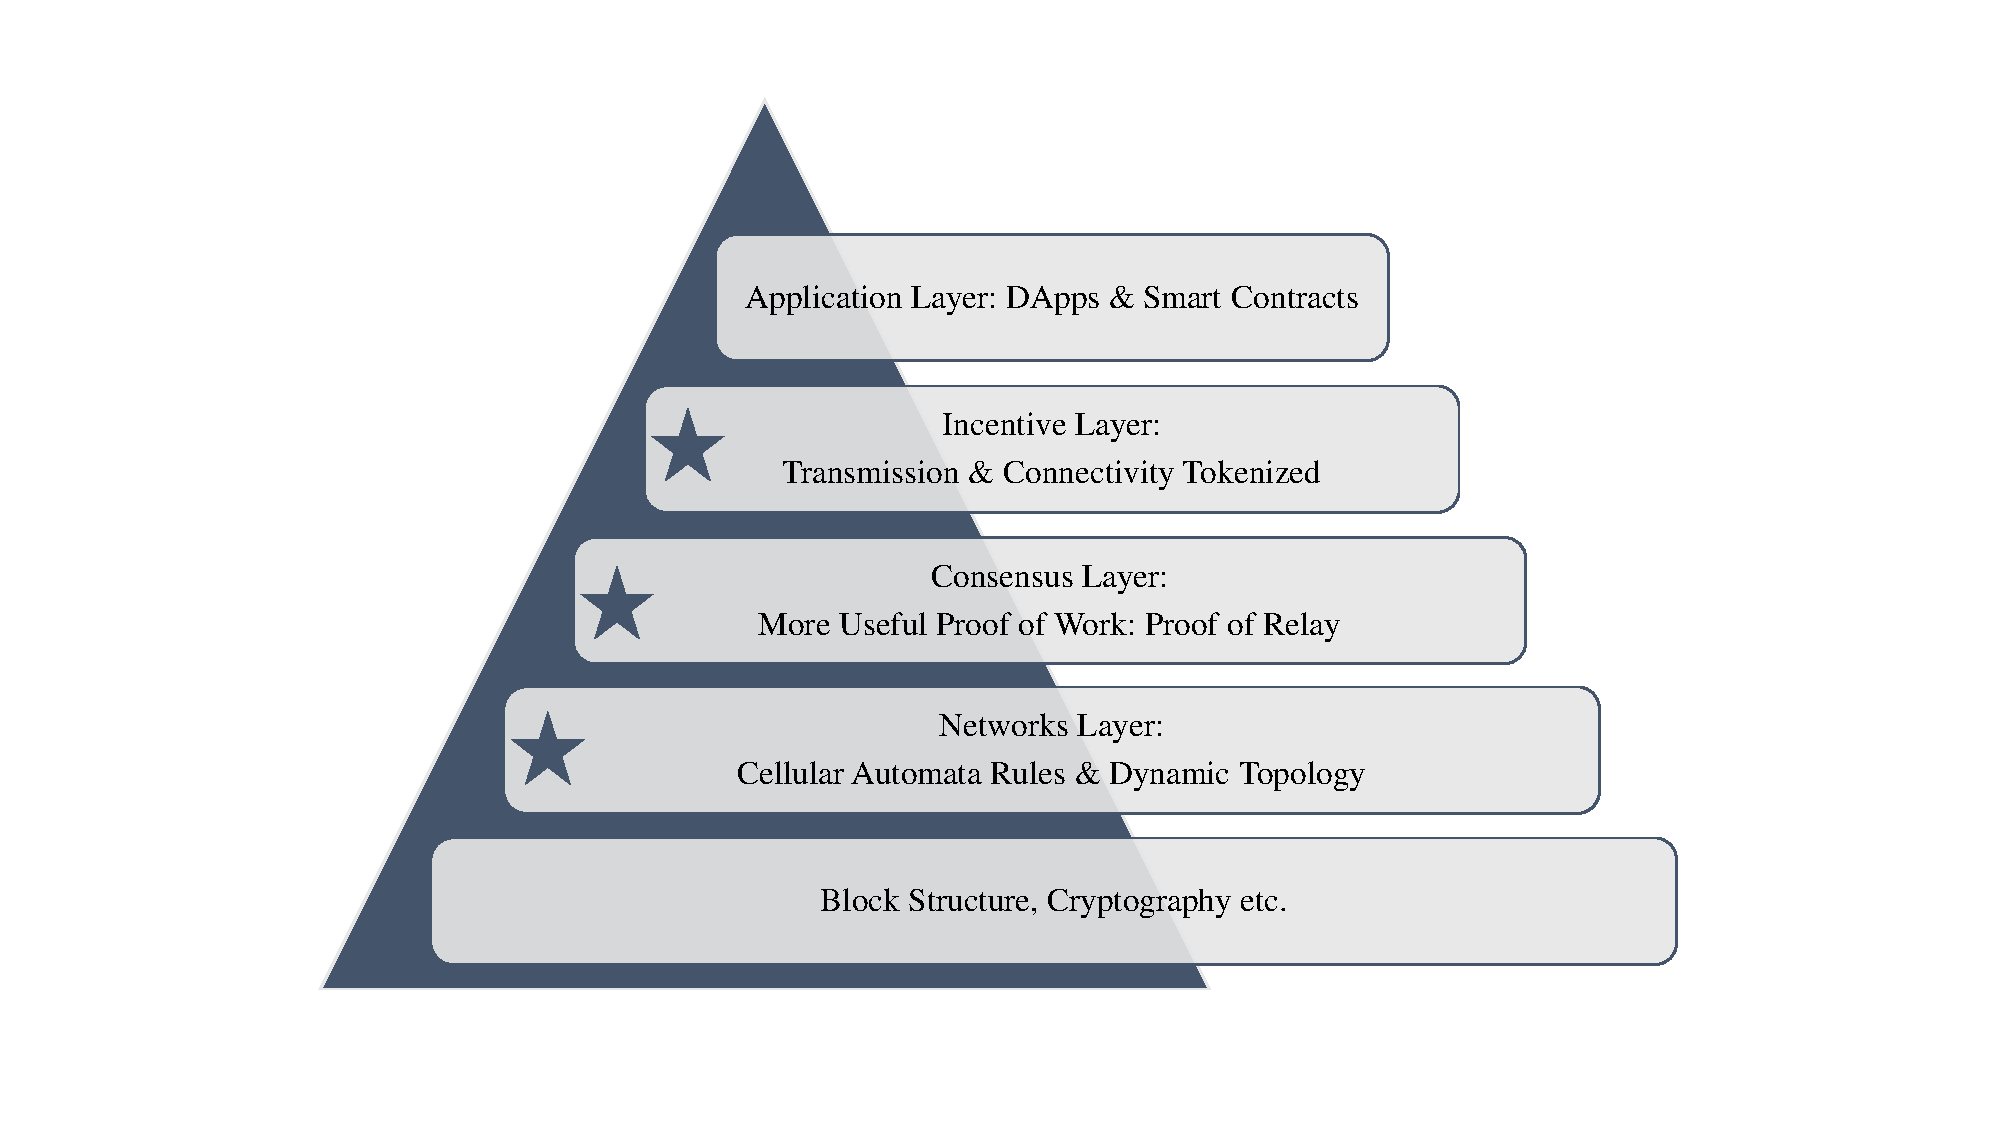
\includegraphics[width=0.9\linewidth]{fig/elementary_components}
\caption{NKN elementary components.}
\label{fig:elementary_components}
\end{figure}

\begin{enumerate}
\item \textbf{Blockchainizing the remaining core building blocks of computing infrastructure}: NKN introduces the concept of decentralized data transmission network (DDTN) scheme and utilizes truly decentralized blockchain to provide network connectivity and data transmission capability by using massive independent relay nodes to solve the problem of precipitation of redundant data on the network.
\item \textbf{Cellular Automata powered DDTN}: NKN introduces the idea of using Cellular Automata to reconstruct the network layer. The intrinsic characteristics of Cellular Automata such as decentralization, peer equivalence and concurrency enable us to build a truly decentralized blockchain network.
\item \textbf{Cellular Automata driven consensus}: NKN achieves consensus efficiently with high fault tolerance in large scale distributed systems based on Cellular Automata, which is essential for decentralized systems without trusted third parties.
\item \textbf{Proof of Relay, A Useful Proof of Work}: NKN proposes Proof of Relay (PoR), a mechanism that encourages participants to contribute to blockchain network by sharing their connectivity and bandwidth to get rewards, enhancing network connectivity and data transmission capacity. PoR is a useful Proof of Work (PoW).
\item \textbf{Tokenization of network connectivity and data transmission capability}: NKN tokenizes network connectivity and data transmission capability by encouraging participants to share their connectivity and bandwidth in exchange for tokens. Idle network resources can be better used through such sharing mechanism. NKN improves the utilization of network resources and the efficiency of data transmission. Refer to our paper on economics model for details \cite{nkn_economic_model}.
\item \textbf{Networking toolkit for fast and painless DApp development}: With NKN, DApp developers now have a new networking toolkit to build truly decentralized applications quickly and easily. DApp developers can focus entirely on creativity, innovation, user interface / user experience and business logic. This networking toolkit is entirely complimentary to the toolkit by other blockchain projects working on identity, machine learning, payment, storage, and etc. 
\end{enumerate}

NKN utilizes Cellular Automata methodologies to achieve full decentralization. All nodes are equal, truly peer to peer, and each is capable of sending, receiving, and relaying data. Cellular Automata makes it possible to have simple local rules that can generate highly dynamical and highly scalable global network overlay topology that is independent of the underlying physical and logical infrastructure. The simplicity and locality of rules make it possible to have cost efficient implementation on all types of network devices, from Internet of Things (IoT), smart phones, all the way to routers. Despite its seemingly simplicity, Cellular Automata enabled routing can be highly random and unpredictable, thus providing superior security and privacy.

NKN nodes get rewarded for providing connectivity and transmission power, resulting in a fully competitive marketplace optimized for maximizing the entire network capacity. For existing networks, NKN will increase the utilization of connectivity and data transmission capacity by sharing the unused bandwidth of participating nodes. More and more new nodes will join the network to earn reward, thus quickly bootstrapping and expanding the NKN network. Existing nodes are incentivized to upgrade and increase data transmission capacity. All of above will further boost overall network capacity, as well as improve the dynamic topology since the network has much more degrees of freedom in choosing the route. 

In addition, NKN proposes a novel and more useful proof of work. Unlike traditional hashing computation type Proof of Work that provides no additional utility, NKN introduces Proof of Relay based on many useful activities including staying on-line for extended period, expanding amount of peer connection, providing high speed and low latency relay, etc. Even the consensus algorithm is designed from ground up to improve efficiency and fairness, while converge deterministically and globally based on local knowledge.

Furthermore, NKN is intended to promote network sharing and network ownership by its users. NKN's economic model and governance model will reflect this in design and in implementation. These technology and economic model innovations complement each other and together will amplify the power of NKN network.

\subsection{Networking toolkit for Fast and Painless DApp Development}

With NKN, DApp developers now have a new networking toolkit to build truly decentralized applications rapidly and painlessly. DApp developers can focus entirely on the ideas and innovation, UI (user interface) /UX (user experience), and business logic that make their product successful to the end users. They no longer need to wade through the wild jungle of blockchain, cryptography, consensus mechanism, identity and security before they even write one line of code for their users.

For example, in traditional app development with centralized SaaS (Software as a Service) offerings, one can host app on cloud computing platforms, store data on cloud storage, use web services for text message, phone call and payment. In the decentralized blockchain world, it is already conceivable today to build a new kind of Facebook by using Ethereum \cite{buterin2014next} /NEO \cite{neo} for computing, IPFS \cite{benet2014ipfs} for storage, and NKN for networking. The beauty of this new paradigm is that users will personally own their identity and data, and can be both consumer and provider in the entire system as well. On top of that, at each layer there are built-in self-incentivized mechanism to maximize the network effect and bootstrap the entire community. 

NKN will be one of the three foundational elements and play a critical role in this decentralized paradigm.

\section{Technology Foundations}

In this whitepaper, we take selective elements of the NKS (New Kind of Science) \cite{wolfram2002new} as inspiration. NKN utilizes microscopic rules based on Cellular Automata to define network topology, achieves self-evolution behaviors, and explores Cellular Automata driven consensus, which is fundamentally different from existing blockchain network layer.

As a powerful tool to study complex systems, Cellular Automaton is closely linked to philosophical categories such as simple and complex, micro and macro, local and global, finite and infinite, discrete and continuous, etc.

\subsection{Cellular Automata}

\begin{figure}[!htp]
\centering
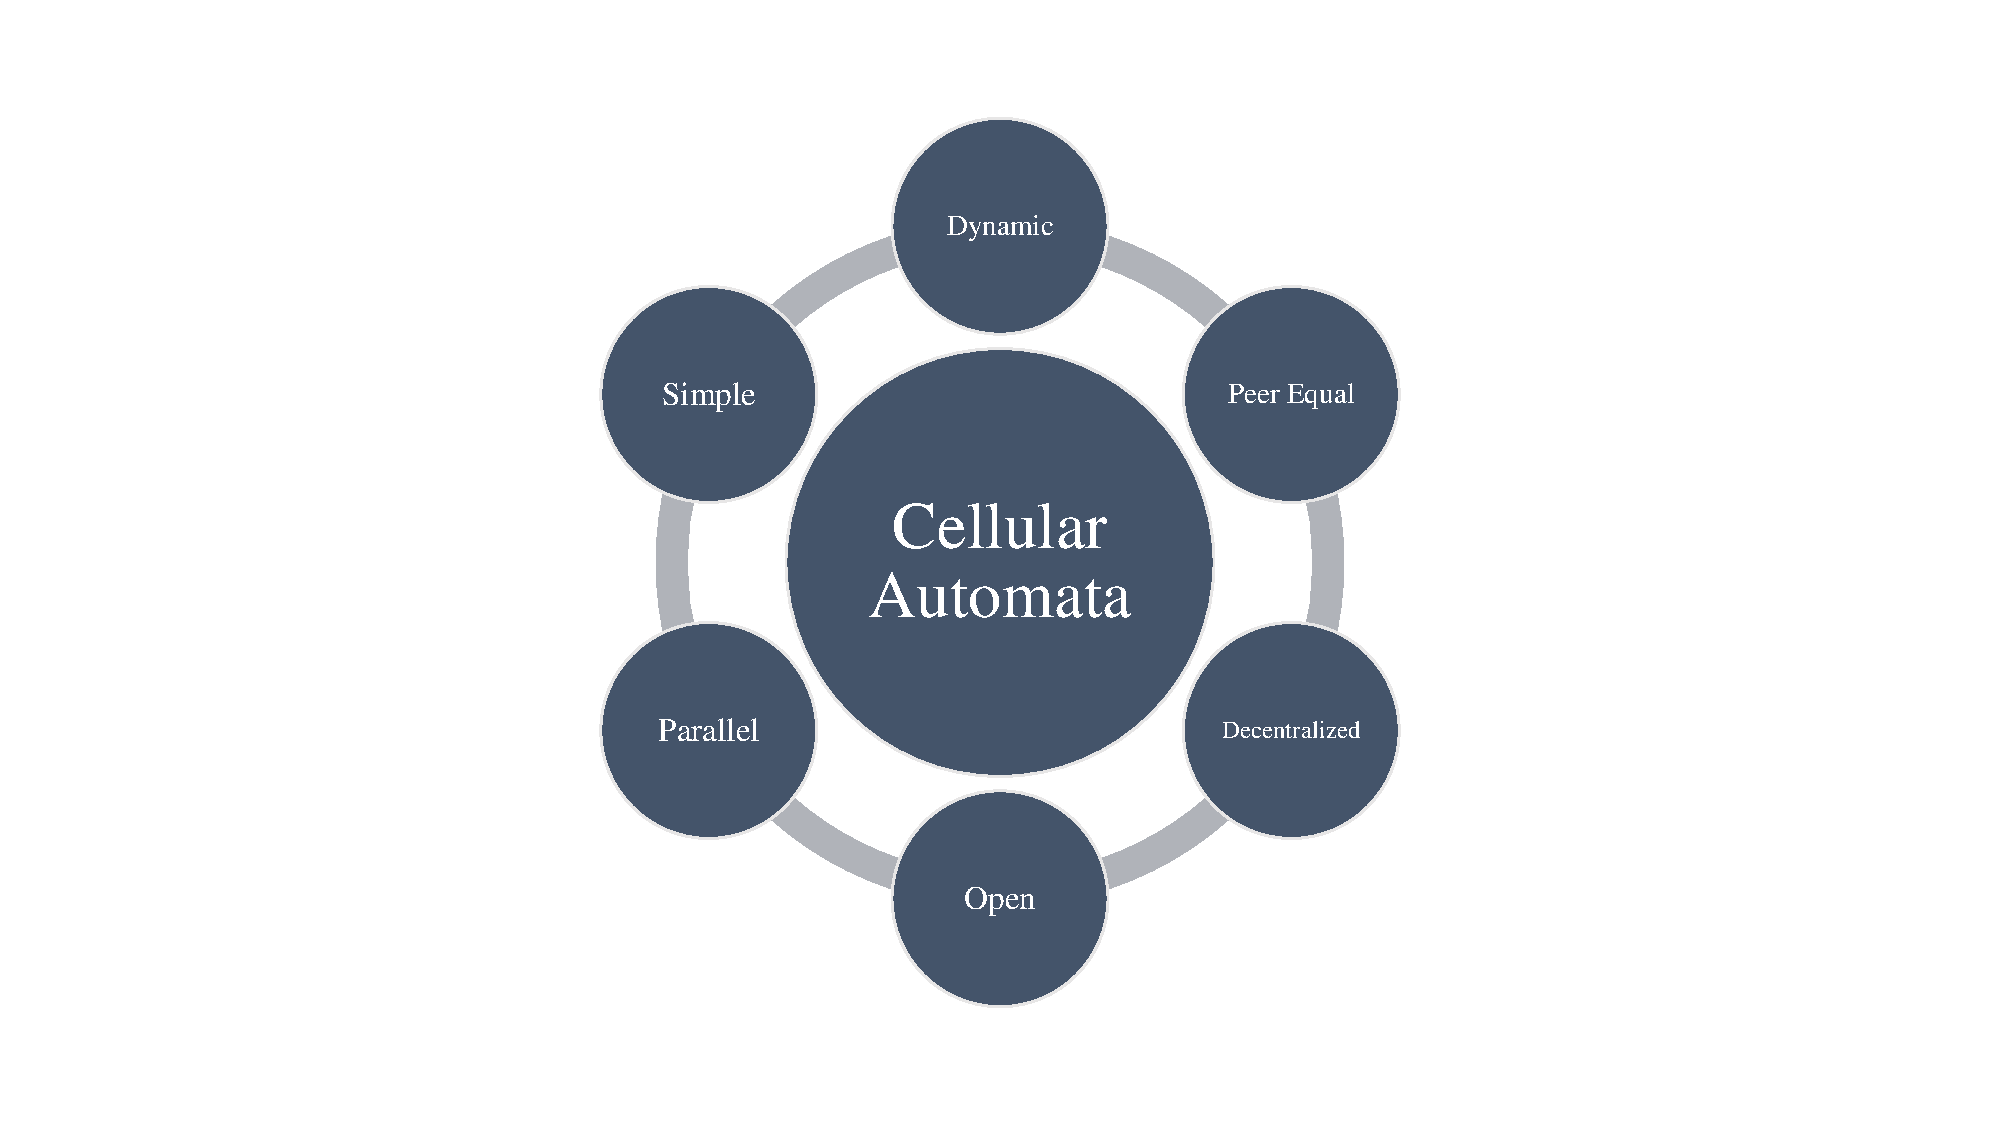
\includegraphics[width=0.7\linewidth]{fig/ca_properties}
\caption{Properties of Cellular Automata.}
\label{fig:ca_properties}
\end{figure}

Cellular Automata (CA) is a state machine with a collection of nodes, each changing its state following a local rule that only depends on its neighbors. Each node only has a few neighbor nodes. Propagating through local interactions, local states will eventually affect the global behavior of CA. The desired openness of network is determined by the homogeneity of Cellular Automata where all nodes are identical, forming a fully decentralized P2P (peer-to-peer) network. Each node in the NKN network is constantly updating based on its current state as well as the states of neighbors. The neighbors of each node are also dynamically changing so that the network topology is also dynamic without changing its underlying infrastructure and protocols.

NKN utilizes CA to achieve efficient, decentralized, and dynamical topology such that information and data can be transmitted efficiently and dynamically without centralized connectivity.

\subsection{Rules as Formulas}

The Cellular Automata programming formula is called ``local rule'', which is an indispensable rule for next generation network of NKN and has an important influence on the network topology \cite{wolfram2002new, yang2007cellular, marr2007regularizing, chung2001diameter, saghiri2017closed}.

Proper choice of local rules leads to Cellular Automata with complex but self-organized behaviors on the boundary between stability and chaos. Rules are essential because they are formulas to program Cellular Automata and Automata Networks. 
The static characteristics of a Cellular Automaton is a discrete dynamic system defined as
\begin{equation}
\text{CA} = (S,N,K,f)
\end{equation}
Finite number of nodes interact in a regular network. $S$ represents states of nodes, where each node has a local state. The state of all nodes determines the global state. $N$ denotes the number of nodes in network. $K$ denotes neighbor set, i.e. which neighbor nodes are taken into account in local state transitions. $f$ denotes a state transition function, which has a dramatic impact on the global evolution of the system.

The dynamic characteristics of a Cellular Automaton is illustrated in Fig.~\ref{fig:ca_characteristics}. Dynamic evolution starts from an initial state. Nodes change their states based on their current states and the states of their neighbor nodes. The global state is fully determined by local states of all nodes and evolves accordingly. 

\begin{figure}[!htp]
\centering
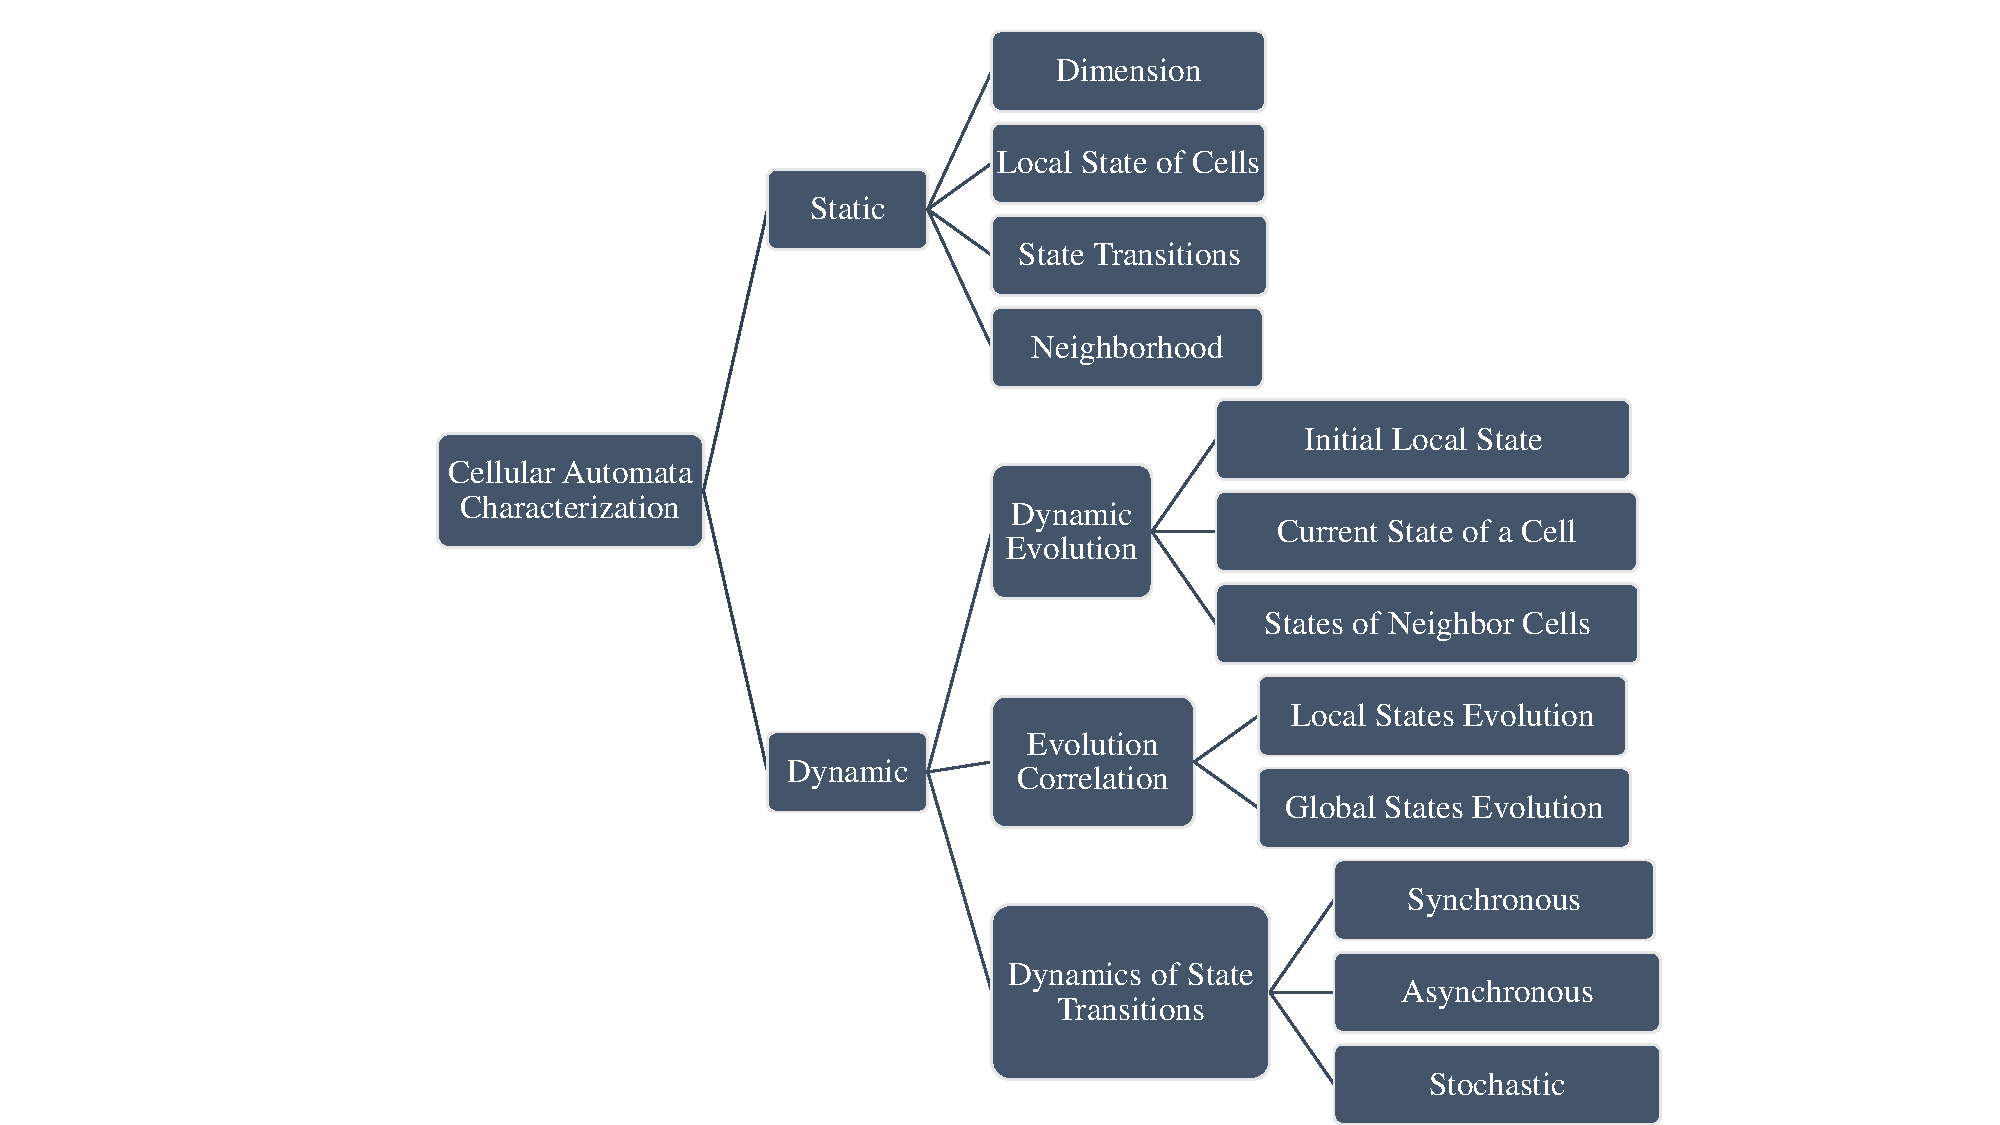
\includegraphics[width=\linewidth]{fig/ca_characteristics}
\caption{Characteristics of Cellular Automata.}
\label{fig:ca_characteristics}
\end{figure}

The NKN team believes CA-based or CA-driven systems are more natural and organic than current approaches utilizing static and fully connected topology. Complex systems with such a simple structure are closer to natural systems, thus enabling self-evolution.

\section{New Kind of Network}

NKN is the next generation of peer to peer network infrastructure built upon blockchain technology backed by Cellular Automata theory aiming at revolutionizing the Internet with true decentralization and native token incentive mechanism.

\subsection{Next Generation Decentralized Network}

As the current leaders in blockchain, Bitcoin and Ethereum tokenize computational power through Proof of Work (PoW). IPFS \cite{benet2014ipfs}, Filecoin \cite{filecoin}, Sia \cite{vorick2014sia} and Storj \cite{wilkinson2014storj}, on the other hand, tokenize storage. Yet, few systems blockchainize network connectivity and data transmission power, the third essential building block in the Internet. NKN is designed to tokenize network connectivity and data transmission capability as a useful PoW.

NKN solves the ``efficiency'' problem of blockchain by equalizing all nodes in the network. Each node follows a rule of Cellular Automaton and updates its state based on local rules. Proposed by Von Neumann in 1940s, Cellular Automaton (CA) is a generic term for a type of model, a state machine characterized by discrete time, space and interaction \cite{von1951general, von1966theory}. It is a discrete system that evolves locally according to specific rules and is proven to be able to emulate the evolution of complex systems. Cellular Automaton has the characteristics of decentralization, peer equality and concurrency. For the first time, NKN proposed Cellular Automata as the fundamental element of the network layer for blockchain, so as to ensure that the entire network layer can benefit from it.

Updating formulas in Cellular Automata are called ``local rules'', which are found to be the critical factor that controls the transition of Cellular Automaton between stability and chaos \cite{wolfram2002new}. As an indispensable part of NKN, rules are one of the main factors impacting the network topology.

NKN introduced the concept of Decentralized Data Transmission Network (DDTN). DDTN combines multiple independent and self-organized relay nodes to provide clients with connectivity and data transmission capability. This coordination is decentralized and does not require trust of any involved parties. The secure operation of NKN is achieved through a consensus mechanism that coordinates and validates the operations performed by each node. DDTN provides a variety of strategies for decentralized application (DApp).

In contrast to centralized network connectivity and data transmission, there are multiple efficient paths between nodes in DDTN, which can be used to enhance data transmission capacity. Native tokens can incentivize the sharing of network resources, and eventually minimize wasted connectivity and bandwidth. Such a property is termed ``self-incentivized''.

\subsection{A Useful Proof of Work}

As the pioneering cryptocurrency, Bitcoin \cite{nakamoto2008bitcoin} is generated by mining, a Proof of Work mechanism that incentivizes miners to verify transactions by solving difficult hashing problems. The downside of Bitcoin mining is that efficient mining requires specialized and expensive hardware and consumes a lot of energy. According to Digiconomist, Bitcoin energy consumption rate is close to 50 TWh/year at mid February 2018 and still increasing, while the number is close to 14 TWh/year for Ethereum. Electricity consumed by these two cryptocurrencies combined has surpassed the electricity usage of many countries.

A way to prove the work while avoiding waste of resources is highly desired. NKN proposes an alternative to the current PoW by providing a more decentralized, dynamically evolving, self-organizing and self-evolving network infrastructure and designing a whole new set of consensus mechanisms. The novel PoW does not result in a waste of resources. Instead, it is a peer-to-peer sharing mechanism at blockchain level. Participants receive rewards by contributing more network resources than they consume. NKN uses Proof of Relay mechanism to guarantee network connectivity and data transmission capacity.

\subsection{Network Topology and Routing}

Cellular Automata on Networks (CAoN) is a natural extension of Cellular Automata \cite{yang2007cellular, marr2007regularizing, smith2011network} that is able to model networks with non-geometric neighbor connections. It is powerful when modeling networks whose topology is evolving based on local rules. As the goal is to build a decentralized blockchain system with dynamic topology, CAoN is a natural model for the system.

We consider a dynamic P2P network with $N$ nodes. The network connections at time $t$ can be described by an $N \times N$ adjacency matrix $A(t)$ that evolves with time. Connections between nodes can be added, removed, or altered at each time step. If the dynamics of $A$ is Markovian, the updating process can be written as
\begin{equation}
A(t+1) = f[A(t)],
\end{equation}
where $f$ is the updating rule of network topology. To keep the updating rule local, $f$ should be chosen such that only information of the neighbors of each node is used when updating its connections. The updating rule above does not contain states of nodes, so the topology evolution is independent of the state of any node. A more general Markovian updating rule should take both topology of the network and states of nodes into consideration such that
\begin{equation}
\begin{aligned}
A(t+1) &= f[A(t), S(t)]\\
S(t+1) &= g[A(t+1), S(t)]
\end{aligned}
\end{equation}
where $S(t)$ is a vector representing the states of all nodes in the network at time $t$, $f$ is the topology updating rule, and $g$ is the state updating rule. Similarly, $f$ and $g$ should be chosen such that only information of current neighbors are used when updating. The state could contain historical information. An example state in blockchain system is all the blocks that a node stores locally. Note that although we describe the system formally using the global state $S$ and global connectivity $A$, each node $i$ only needs to know and store its local state $S_i$ and neighbors $\{ j | A_{ij} \neq 0 \}$.

Consider a CAoN in a blockchain system where blocks are being generated. Each time a block is received, the node updates its state and send the block to neighbors with digital signature. The neighbors will decide whether to forward the message depending on their states like if it has received the block, if the block is valid, or conflict with other block in state, effectively affecting the topology of the entire network without changing the physical layer or the underlying protocol.

As an example to illustrate how we model the network, one can consider a general Network Automaton that allows an arbitrary number of neighbors. For simplicity, a minimalist approach is adopted to emulate blockchain expanding and data relay from a small set of microscopic rules. Initially (at time zero) the network is a 3D cubic structure with 8 nodes, each has 3 neighbors, as shown in Fig.~\ref{fig:ca_blockchain_node}.

\begin{figure}[!htp]
\centering
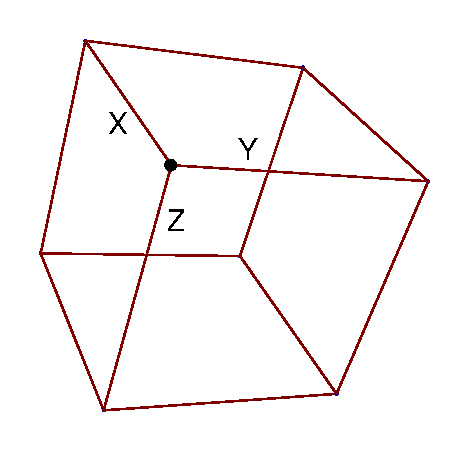
\includegraphics[width=0.5\linewidth]{fig/ca_blockchain_node}
\caption{An example of Network Automata with 8 nodes forming a cubic network in 3D space at initial state.}
\label{fig:ca_blockchain_node}
\end{figure}

Starting from the simple network in Fig.~\ref{fig:ca_blockchain_node}, the system is extended by adding nodes to it following various updating rules. The resulting topology can be dramatically different when different rules are used, as shown in Fig.~\ref{fig:ca_blockchain_topology}.

\begin{figure}[!htp]
\centering
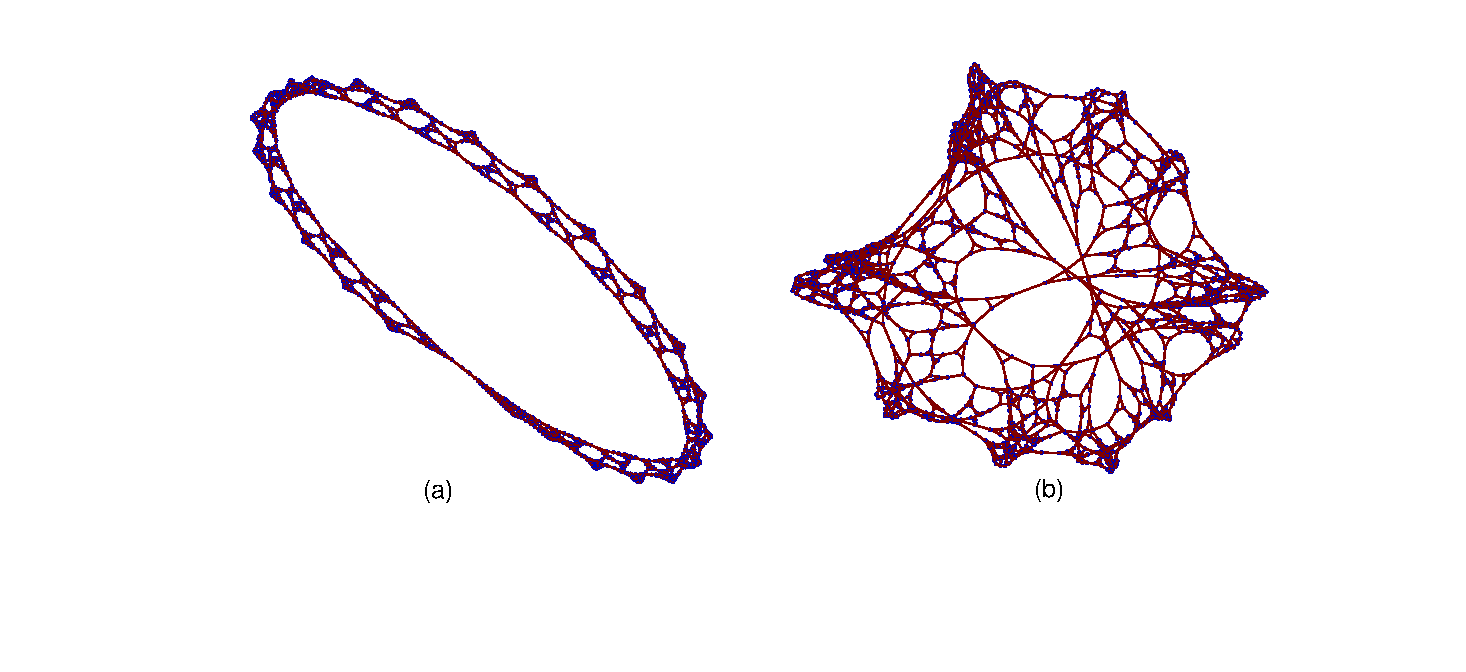
\includegraphics[width=0.9\linewidth]{fig/ca_blockchain_topology}
\caption{Some examples of complex blockchain network topologies with various simple rule sets (a) ring topology, rule 1655146, time step 1573; (b) pseudo-random topology, rule 1655185, time step 1573.}
\label{fig:ca_blockchain_topology}
\end{figure}

NKN will bridge network evolution and blockchain functions using similar network models with microscopic rules. The simple local rules make replication straightforward, simplifying and accelerating system implementations.

\subsubsection{Dynamics}

Dynamics in CAoN are purely local: each node evaluates the state transition independently of other nodes and changes its state accordingly \cite{chopard1998cellular}. Node state can be driven by either the interaction between nodes, or external information, as shown in Fig.~\ref{fig:node_change_state_condition}.

\begin{figure}[!htp]
\centering
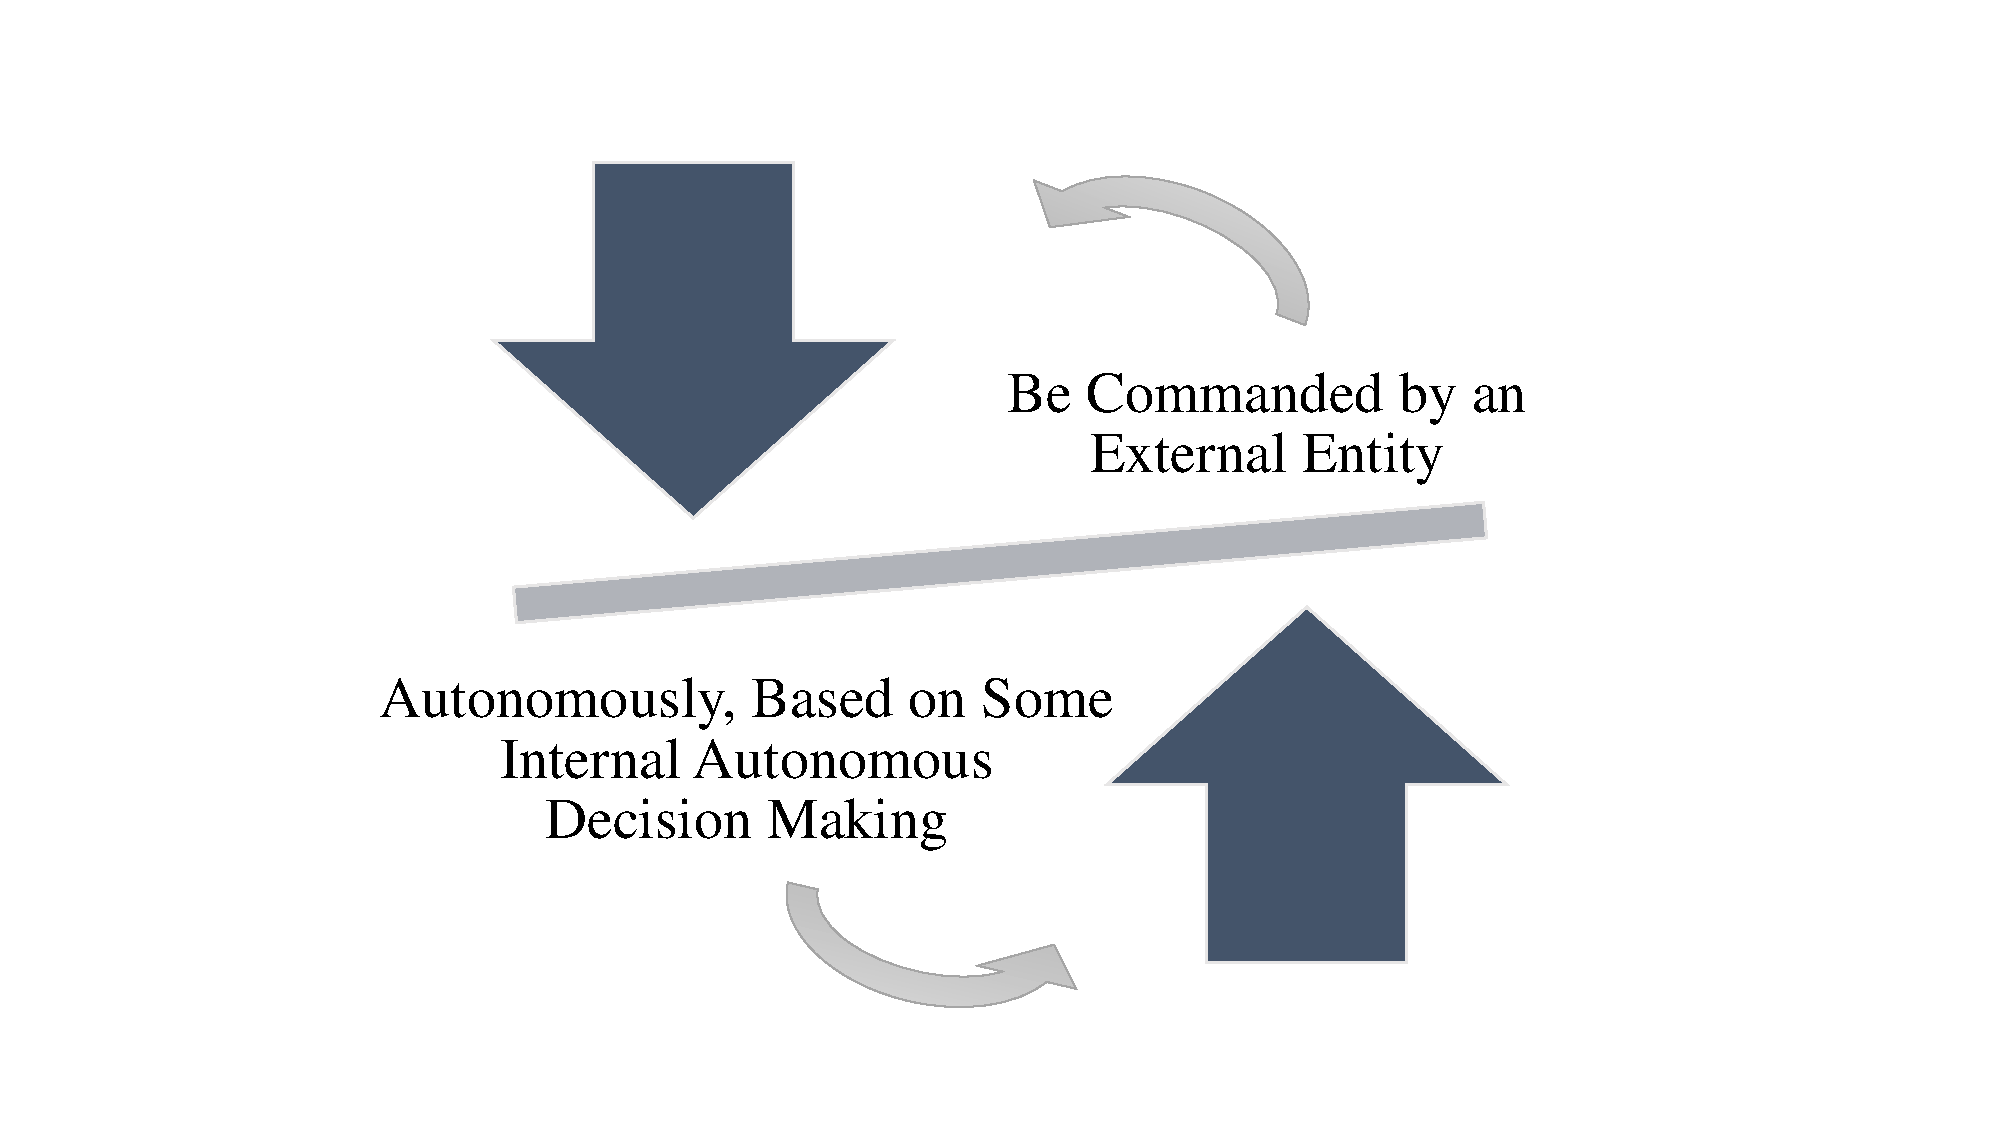
\includegraphics[width=0.7\linewidth]{fig/node_change_state_condition}
\caption{Possible conditions for a node to change its state in CAoN.}
\label{fig:node_change_state_condition}
\end{figure}

Rules are crucial to the resulting topology in CAoN. Network topology would be very different given small changes in the updating rules, as shown in Fig.~\ref{fig:ca_network_dynamics}.

\begin{figure}[!htp]
\centering
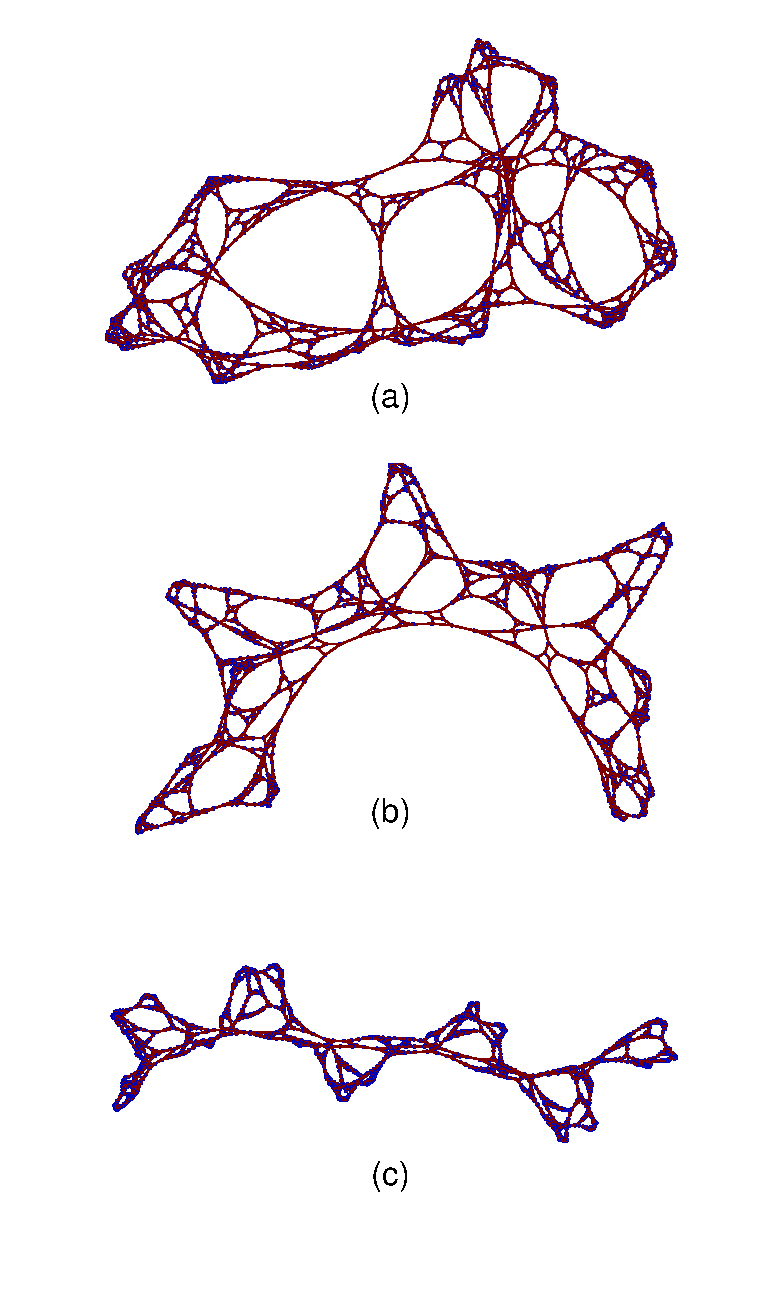
\includegraphics[width=0.6\linewidth]{fig/ca_network_dynamics}
\caption{Dynamics of network topology by rewriting rules of Cellular Automata at the same time step index, (a) rule 1655163, time step 1573; (b) rule 1655175, time step 1573; (c) rule 1655176, time step 1573.}
\label{fig:ca_network_dynamics}
\end{figure}

Although in the mathematical description discrete time step was used for convenience, CAoN does not require nodes have any global time or discrete time. Instead, each node performs the update asynchronously \cite{chopard1998cellular}. This is a more general and realistic description of real blockchain networks.

\subsubsection{Self-Organization}

The global dynamics of Cellular Automata can be classified into 4 types \cite{wolfram2002new}: steady, periodic, chaotic, and complex. Our focus is in the complex type (Class 4), also known as the “edge of chaos”, where all initial patterns evolve into structures that interact in complex ways, with the formation of local structures that can survive for long periods of time. Wolfram speculates that although not all of the Class 4 Cellular Automata are capable of universal computation, many of them are Turing-complete. This view has been successfully proven by the Rules 110 \cite{wolfram2002new, cook2004universality} and Conway's Game of Life \cite{conway1970game}. Complex, self-organizing and dynamical structures emerge spontaneous in Class 4 CA, providing us an ideal candidate for the basis of decentralized systems.

\begin{figure}[!htp]
\centering
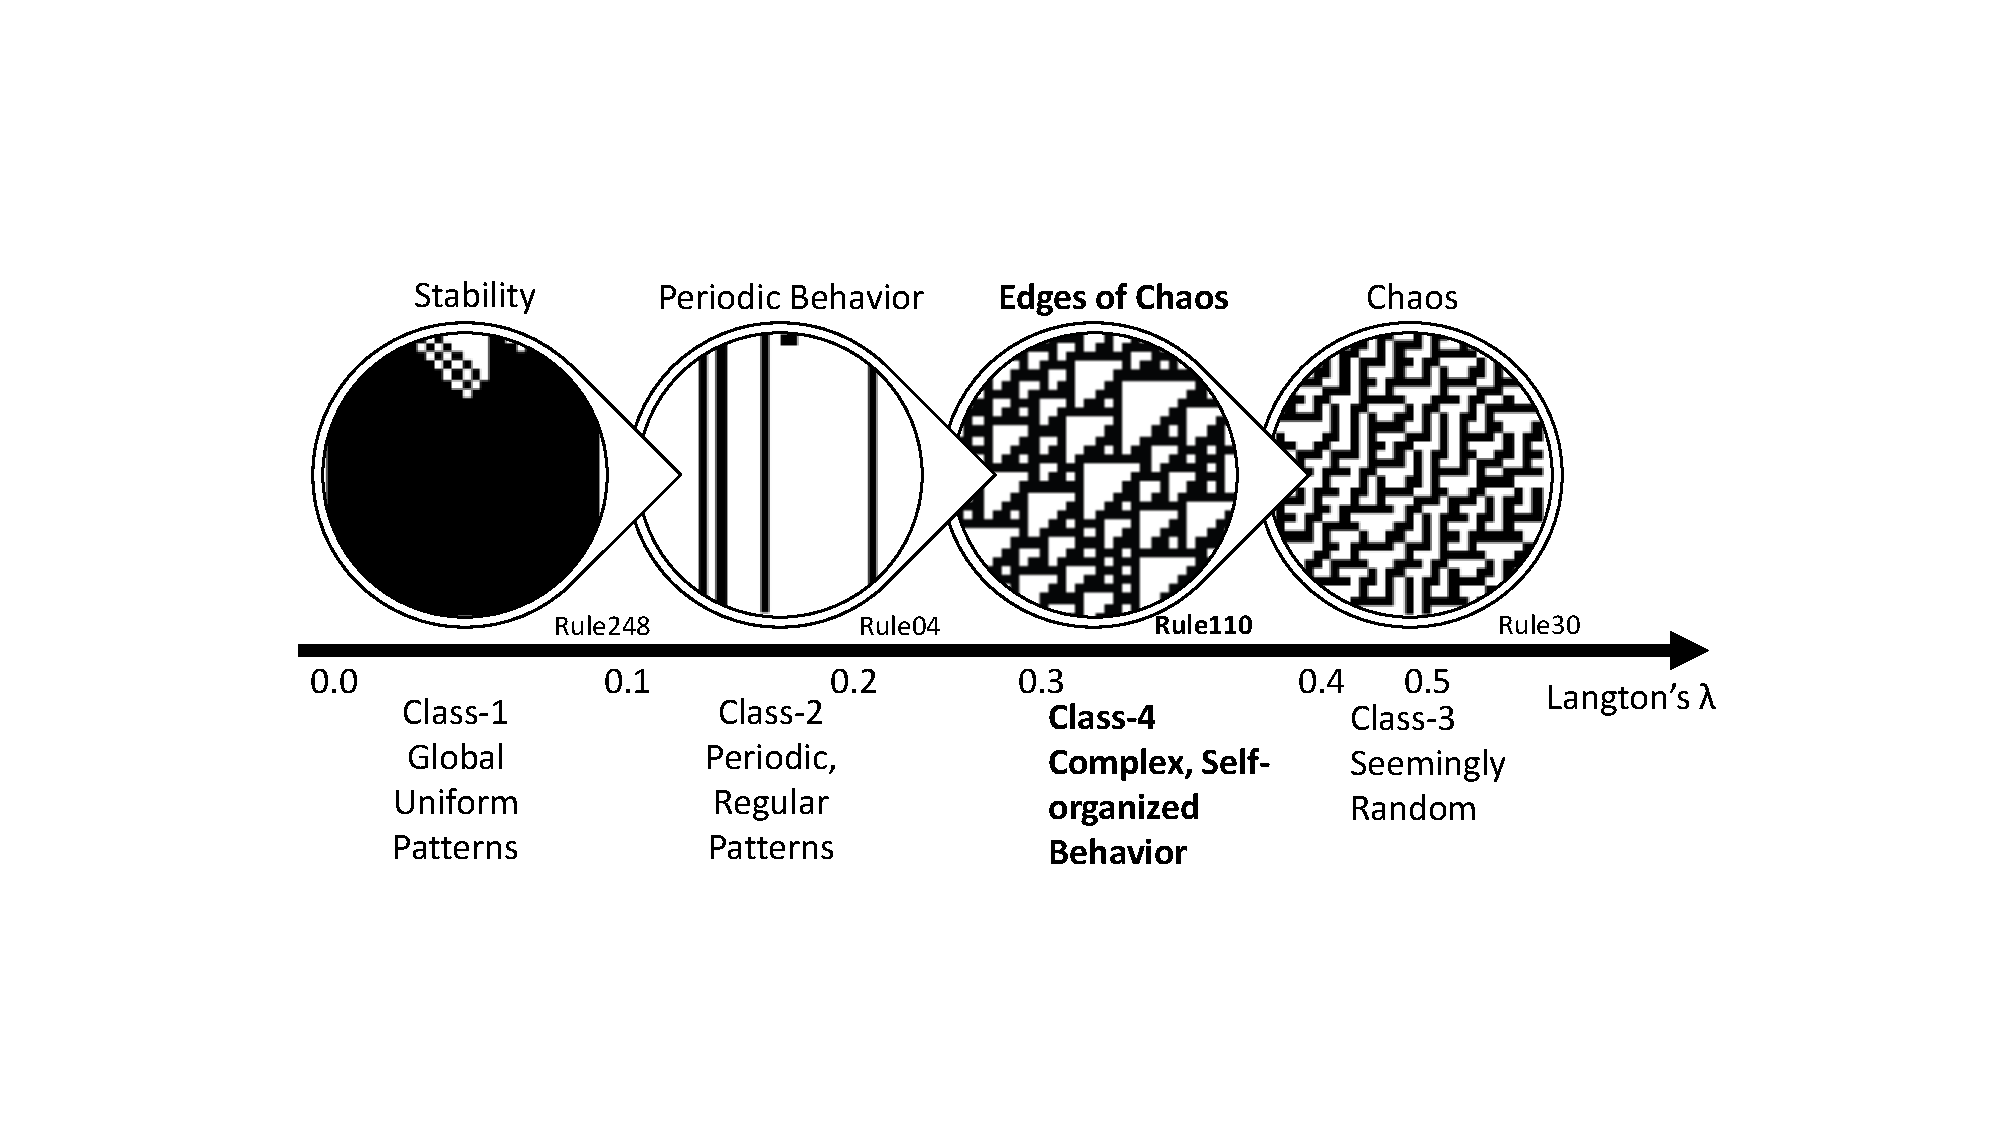
\includegraphics[width=\linewidth]{fig/ca_classes_lambda}
\caption{Wolfram's 4 classes of behaviors versus Langton's $\lambda$ parameter on 1D Cellular Automata.}
\label{fig:ca_classes_lambda}
\end{figure}

A quantitative measure of the rule that can explain and predict the behavior type of the CA is the Langton's $\lambda$ parameter defined by the fraction of rule table entries that results in active state. As $\lambda$ increases from 0, the system will transit from steady state to periodic state, then to complex state, and finally to chaos state, as shown in Fig.~\ref{fig:ca_classes_lambda}. In the classic 1D CA with nearest neighbor interaction, Class 4 behavior emerges when $\lambda$ is around 0.3. Langton's $\lambda$ parameter provides us a theoretical guide on how to find the desired updating rules, which is essential for high dimensional systems.

\subsubsection{Self-Evolution}

CAoN is inherently self-evolving due to its simple but powerful local dynamics. The updating rule essentially sets the direction of evolution, and the system evolves continuously towards the direction, regardless of the initial states or how nodes are added to the network. Fig.~\ref{fig:ca_evolution} shows an example of the self-evolution in CAoN.

\begin{figure}[!htbp]
\centering
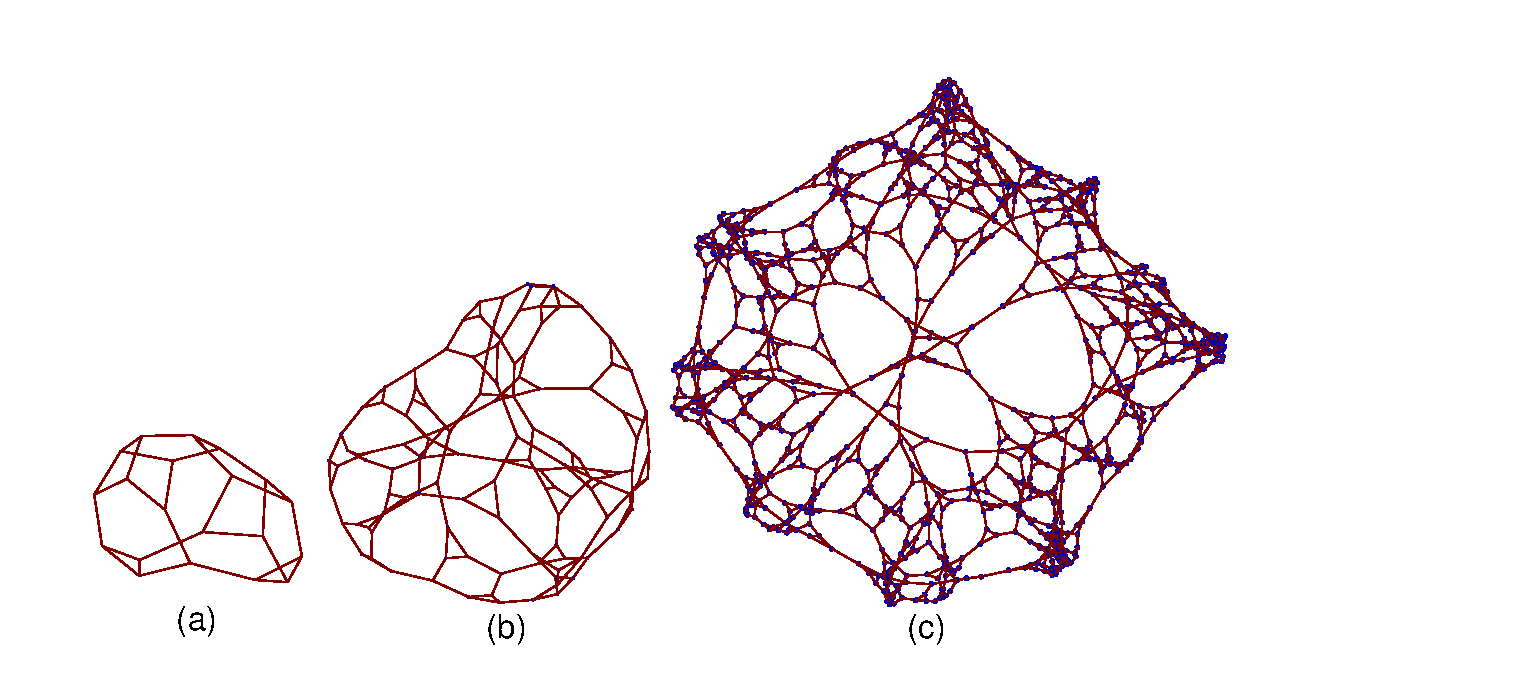
\includegraphics[width=0.9\linewidth]{fig/ca_evolution}
\caption{Self-evolution of a 3D CAoN model on rule 1655185 at various time step index (a) 100; (b) 1000; (c) 10000.}
\label{fig:ca_evolution}
\end{figure}

\subsection{Efficient Decentralization}

Due to the dynamical nature of NKN, network topology between nodes is constantly updating. Proper updating mechanism is critical to achieve decentralization of the resulting topology. If, for example, the updating mechanism is chosen such that a newly joined node has higher chance to choose node with more neighbors to be its neighbor, and the probability to choose a node is proportional to the degree of that node, then the resulting network will be scale-free \cite{barabasi1999emergence}: the degree distribution follows a power law form. Such networks have “centralized” hubs defined by nodes with huge degree. Although hubs could potentially increase efficiency, they make network less robust as the failure of hubs will have much larger impact than the failure of other nodes. 

One of the NKN's goals is to design and build networks that are decentralized while still being efficient in information transmission. This should be done by using a proper topology updating mechanism that considers both algorithm and incentive. On the algorithm side, neighbors should be sampled and chosen randomly; on the incentive side, reward for data transmission should be sublinear (grows slower than linear function) so that hubs are discouraged. Sparse random network is one possible topology that could be generated from such mechanism. It is decentralized and thus robust to the failure of any node, while still being efficient in routing due to its small network diameter \cite{chung2001diameter}.

\section{Cellular Automata Powered Consensus}

Nodes in blockchain are peers due to the decentralized nature of blockchain. The inherent lack of trust in blockchain systems is particularly noteworthy because any node can send any information to any nodes in the blockchain. Peers must evaluate information and make agreement on their actions for blockchain to work properly \cite{baliga2017understanding}.

NKN is designed to be a futuristic blockchain infrastructure that requires low latency, high bandwidth, extremely high scalability and low cost to reach consensus. These properties are crucial for future DApps. Thus, NKN needs new consensus algorithms that could satisfy such high requirements.

\subsection{Mainstream Consensus}

Currently there are several approaches to reach consensus in blockchain: Byzantine fault tolerance algorithm (BFT) \cite{lamport1982byzantine}, practical Byzantine fault tolerance algorithm (PBFT) \cite{castro2002practical}, Proof of Work algorithm (PoW) \cite{nakamoto2008bitcoin}, proof of stake algorithm (PoS) \cite{vasin2014blackcoin, king2012ppcoin}, and delegated Proof of Stake algorithm (DPoS) \cite{dpos}.

\begin{enumerate}
\item \textbf{Practical Byzantine Fault Tolerant (PBFT)}: Byzantine fault tolerance is a model that Leslie Lamport proposed in 1982 to explain the issue of consensus. It discusses the consensus under the scenario where some nodes could be evil (the message may be forged) and provides a worst-case guarantee \cite{lamport1982byzantine}. In Byzantine fault tolerance, let the total number of nodes be $N$ and the number of bad nodes be $F$, If $N \geq 3F + 1$, then the problem can be solved by the Byzantine Fault Tolerant (BFT) algorithm. Lamport proved that there is a valid algorithm such that when the fraction of bad nodes does not exceed one-third, good nodes could always reach consensus no matter what messages bad nodes send. Practical Byzantine Fault Tolerant (PBFT), first proposed by Castro and Liskov in 1999, was the first BFT algorithm to be widely used in practice \cite{castro2002practical}. PBFT is much more efficient and works in an asynchronized way, while it can still tolerate same number of faulty nodes as BFT, making it more practical to use in real systems.
\item \textbf{Proof of Work (PoW)}: Bitcoin blockchain network introduced an innovative Proof of Work (PoW) algorithm \cite{nakamoto2008bitcoin}. The algorithm limits the number of proposals by increasing the cost of them, and relax the need for final confirmation of conformity by agreeing that everyone will accept the longest-known chain. In this way, anyone who tries to vandalism will pay a great economic cost. That is, to pay more than half the system computing power. Later, various ``PoX'' series algorithms are proposed following this thought, using economic penalties to restrict the spoilers. PoW is the consensus used by Bitcoin and is also the earliest used in blockchain system. In brief, PoW means how much work a miner pays and how much it gains. The work here is the computing power and time which a miner provides contribute to the blockchain system. The process of providing such services is ``mining''. In PoW, the mechanism to allocate reward is that the mining income is proportional to the computing power. The more powerful mining machine used, the more expected reward miners will get.
\item \textbf{Proof of Stake (PoS)}: Initially, Proof of Stake reduces the difficulty of calculating hash according to the amount of tokens held. PoS is similar to financial assets in bank, which distribute financial return proportional to the amount of assets that stakeholder holds in a given period. Similarly in PoS, the blockchain system allocates ``interests'' according to stakeholder's token amount and hold time \cite{vasin2014blackcoin, king2012ppcoin}. In Delegated Proof of Stake (DPoS), not every stakeholder is able to create block. Instead, nodes vote for trustees that represent them to enter the “parliament” and create blocks. Users who would like to become trustees need to go through community canvassing in order to gain trust of the community \cite{dpos}.
\end{enumerate}

\subsection{Cellular Automata Powered Consensus}

\subsubsection{Scalability Issue of BFT and PBFT}

It is challenging to get consensus in large distributed systems using BFT and PBFT algorithm. In BFT algorithm, the total number of messages to be sent in the system is $O(N!)$\cite{lamport1982byzantine}, making it not practical. PBFT algorithm reduced the total message count to $O(N^2)$\cite{castro2002practical}, which is tractable but not scalable when $N$ is large. In addition, both BFT and PBFT requires every node to have a list of all other nodes in the network, which is hard for dynamical network.

\subsubsection{Consensus in Cellular Automata Described by Ising Model}

Cellular Automata (CA) is naturally a large distributed system with only local connections. The asymptotic behavior of the system is controlled by its updating rule. It is possible to achieve guaranteed global consensus in CA using message passing algorithm based only on sparse local neighbors for a set of updating rules. 

Using the mathematical framework originally developed for Ising model \cite{ising1925beitrag} in physics, we found and proved that a class of CA rules will guarantee to reach consensus in at most $O(N)$ iterations using only states of sparse neighbors by an exact map from CA to zero temperature Ising model. Some studies investigated the fault tolerance of Cellular Automata and how to increase robustness in Cellular Automata-Based systems \cite{mccann2008fault, vzaloudek2011increasing, ccapuni2012turing}. We further showed that the result is robust to random and malicious faulty nodes and compute the threshold when desired consensus cannot be made.

\subsubsection{Ising Model}

Ising model is a model of spin systems with pairwise interaction under external magnetic field \cite{ising1925beitrag}. The Hamiltonian (energy) of the system without external magnetic field can be written as
\begin{equation}
H(s) = -\sum_{i, j} J_{ij} s_i s_j,
\end{equation}
where $s_i = \pm 1$ is the spin of node $i$, and $J_{ij}$ is the interaction between node $i$ and node $j$. We consider the case where $J_{ij}$ can only be 1 (ferromagnetic interaction) or 0 (no interaction). The probability that the system will be in state $s$ under equilibrium follows the Boltzmann distribution
\begin{equation}
p(s) = \frac{1}{Z} e^{-\beta H(s)} = \frac{1}{Z} e^{\beta \sum_{i, j} J_{ij} s_i s_j},
\end{equation}
where $Z = \sum_s e^{-\beta H(s)}$ is the partition function, $\beta = \frac{1}{k_B T}$ with $k_B$ being Boltzmann constant and $T$ being the temperature, representing noise level of the system. The units where $k_B = 1$ will be used for simplicity.

Ising model on lattice has been extensively studied \cite{ising1925beitrag, onsager1944crystal}. For the Ising model on a $D$ dimensional lattice with nearest neighbor interaction, a phase transition occurs at finite critical temperature $T_c$ except for $D = 1$ where the critical temperature $T_c = 0$. When $T < T_c$, the system collapse into one of the two states where nodes have a preferred spin (spontaneous magnetization), while the system does not have a preferred spin when $T > T_c$.

For example, for a 2D square lattice with nearest neighbor interaction, the exact solution of the Ising model can be obtained. The critical temperature is
\begin{equation}
T_c = \frac{2}{\ln(1 + \sqrt{2})} \approx 2.27,
\end{equation}
and the spontaneous magnetization is
\begin{equation}
\langle s \rangle = \pm \left[ 1 - (\sinh{2\beta})^{-4} \right]^{\frac{1}{8}}.
\end{equation}
All of the spins will become the same (either 1 or -1) when $T \to 0$.

If the distributed system of interest can be mathematically described by an Ising model, then the system is guaranteed to achieve consensus (all nodes have the same states) when temperature is zero. Finite temperature plays the role of failure by adding randomness to state transition, and finite critical temperature leads to robustness to such failure.

\subsubsection{Link Between Cellular Automata and Ising Model}

Cellular Automata (CA) is closely related to Ising Model. A CA is characterized by its updating rule
\begin{equation}
p(s^{t+1} | s^t) = \prod_i p(s^{t+1}_i | s^t)
\end{equation}
that represents the probability of the system to transfer to state $s^{t+1}$ at time $t + 1$ given system state $s^t$ at time $t$. The transfer probability is conditional independent because every node in CA updates its state solely depending on the previous system state. For deterministic CA, the transfer probability $p(s^{t+1} | s^t)$ is a delta function. If a Hamiltonian of the form $H(s) = -\sum_{i,j} J_{ij} s_i s_j$ can be defined for a CA such that
\begin{equation}
p(s^{t+1}_i | s^t) \propto e^{-\beta H(s^{t+1}_i | s^t)} = e^{\beta \sum_j J_{ij} s^{t+1}_i s^t_j},
\end{equation}
where $H(s^{t+1}_i | s^t)$ is the Hamiltonian of the system given state $s_j = s^t_j, \forall j \neq i$ and $s_i = s^{t+1}_i$. The transfer probability becomes
\begin{equation}
p(s^{t+1} | s^t) \propto e^{\beta \sum_{i,j} J_{ij} s^{t+1}_i s^t_j}.
\end{equation}

We now define a new state $S^t$ which is a joint state of $s^{t-1}$ and $s^t$ such that $p(S^t) \equiv p(s^{t-1}, s^t)$. The transfer probability of $S^t$ is now proportional to the Boltzmann distribution
\begin{equation}
p(S^{t+1} | S^{t}) = p(s^{t+1} | s^t) \propto e^{\beta \sum_{i,j} J_{ij} s^{t+1}_i s^t_j} = e^{-\beta H(S^{t+1})},
\end{equation}
with Hamiltonian $H(S^t) \equiv -\sum_{i,j} J_{ij} s^{t-1}_i s^t_j$ where the interaction within $s^t$ and within $s^{t-1}$ is zero. Thus, the CA is mapped to an Ising model with state $S$. The stationary distribution of $S$ follows the Boltzmann distribution
\begin{equation}
p(S) = \frac{1}{Z} e^{-\beta H(S)},
\end{equation}
while the stationary distribution of $s$ is given by
\begin{equation}
p(s) = \frac{1}{Z} \sum_{s^*} e^{\beta \sum_{i,j} J_{ij} s_i s^*_j}
\end{equation}

Deterministic CA can be mapped to Ising model at zero temperature, where $T \to 0$, $\beta \to \infty$, $p(S)$ and $p(s)$ is nonzero only at state(s) with lowest energy. In the case of $J_{ij} = 1$ or $0$ which we are interested in, only two states ($s_i = 1, \forall i$ or $s_i = -1, \forall i$) are allowed at zero temperature.

\subsubsection{Majority Vote Cellular Automata as a Consensus Algorithm}

Majority Vote Cellular Automata (MVCA) is a Cellular Automata using majority vote as updating rule. It can be formalized as
\begin{equation}
s^{t+1}_i = \text{sign} \left( \sum_j J_{ij} s^t_j \right),
\end{equation}
where $J_{ij} = 1$ if node $i$ and $j$ are connected, otherwise $0$. $\text{sign}(x) = 1$ if $x > 0$, or $-1$ if $x < 0$. $\text{sign}(0) = 1$ or $-1$ with equal probability. The definition of $\text{sign}(0)$ does not have any impact if each node has odd number ($k$) of connections, which is true for $D$ dimensional Cellular Automata with nearest neighbor connections and self connection. Only odd $k$ is considered for simplicity.

The Hamiltonian can be defined as $H = -\sum_{i,j} J_{ij} s_i s_j$. One can check that the majority vote rule satisfies the mapping condition $p(s^{t+1}_i | s^t) \propto e^{\beta \sum_j J_{ij} s^{t+1}_i s^t_j}$ with zero temperature ($\beta \to \infty$). According to the previous section, when MVCA reaches equilibrium, all nodes will have the same state which depends on initial condition.

To show that MVCA will converge to its equilibrium, we use the equation derived in previous section $p(S^{t+1} | S^{t}) \propto e^{-\beta H(S^{t+1})}$. Since $\beta \to \infty$, $p(S^{t+1} | S^{t})$ is nonzero only when $H(S^{t+1})$ is minimized. From the definition of $H(S)$ we get $ -\sum_{i,j} J_{ij} s^{t+1}_i s^t_j \leq -\sum_{i,j} J_{ij} s_i s^t_j, \forall s_i$, where equal is possible only when $s^{t+1} = s$ since $s^{t+1}$ is uniquely determined by $s^t$ when every node has odd number of connections. Specifically, for $s = s^{t-1}$ we have $H(S^{t+1}) \leq H(S^t)$, where equal holds only when $s^{t+1} = s^{t-1}$, i.e. system in equilibrium or two state oscillation. The latter one can be avoided when $J$ is dynamic so we ignore it for now. So $H(S^{t+1}) < H(S^t)$ before MVCA reaches its equilibrium. On the other hand, we note that $H(S)$ can only be integers that change in step of 2 and $-kN \leq H(S) \leq kN$, where $N$ is the total number of nodes in the system and $k$ is the number of connections each node has. Thus MVCA guarantees to converge to consensus state in at most $kN$ iterations for any initial state. Similarly, if the initial state has $m$ ``incorrect'' values, it takes at most $km$ iterations to correct those ``incorrect'' values.

Although in the derivation above we use CA as the model, we did not assume local connectivity. In fact, the results are valid for any network topology with symmetric connectivity matrix $J$.

\subsubsection{Randomized Neighbors}

Cellular Automata and Ising model are both lattice based system with interaction strength mostly depends on Euclidean distance. Such kind of models are mathematically easier to solve, while not practical to implement in distributed systems, especially when nodes are dynamical, unreliable, and uncontrollable. Here we propose that random network should be a better topology for consensus in distributed system with dynamical nodes. The consensus algorithm we proposed works in random networks without any modification so that every node does not need to maintain a specific connectivity. It should be mentioned that the random network discussed here is purely an overlay network, regardless of how the nodes are physically connected. In a distributed system where node does not have a list of other nodes, one can use algorithms like peer sampling to achieve random connectivity.

A critical parameter that controls how fast information propagates and thus consensus could be made is the network diameter which is defined as the shortest distance between the two most distant nodes in the network. For a random network where each node has $k$ neighbors and $k$ is $O(log N)$, the diameter of the network is at most $O(log N)$ \cite{chung2001diameter}, much smaller than a lattice based system. This is expected since random network could have “long range” connections, which is not possible in lattice systems. As a result, random networks converge faster to consensus states. It is also shown that increase $k$ leads to smaller diameter \cite{chung2001diameter}, as one may expect.

Wolfram Class 4 Cellular Automata is ideal to construct the randomized network for superior consensus performance. In Class 4 CA, the connectivity is effectively unpredictable, self-organized and self-evolved.

\subsubsection{Simulations of CA Consensus Algorithm}

\begin{figure*}[!htp]
\centering
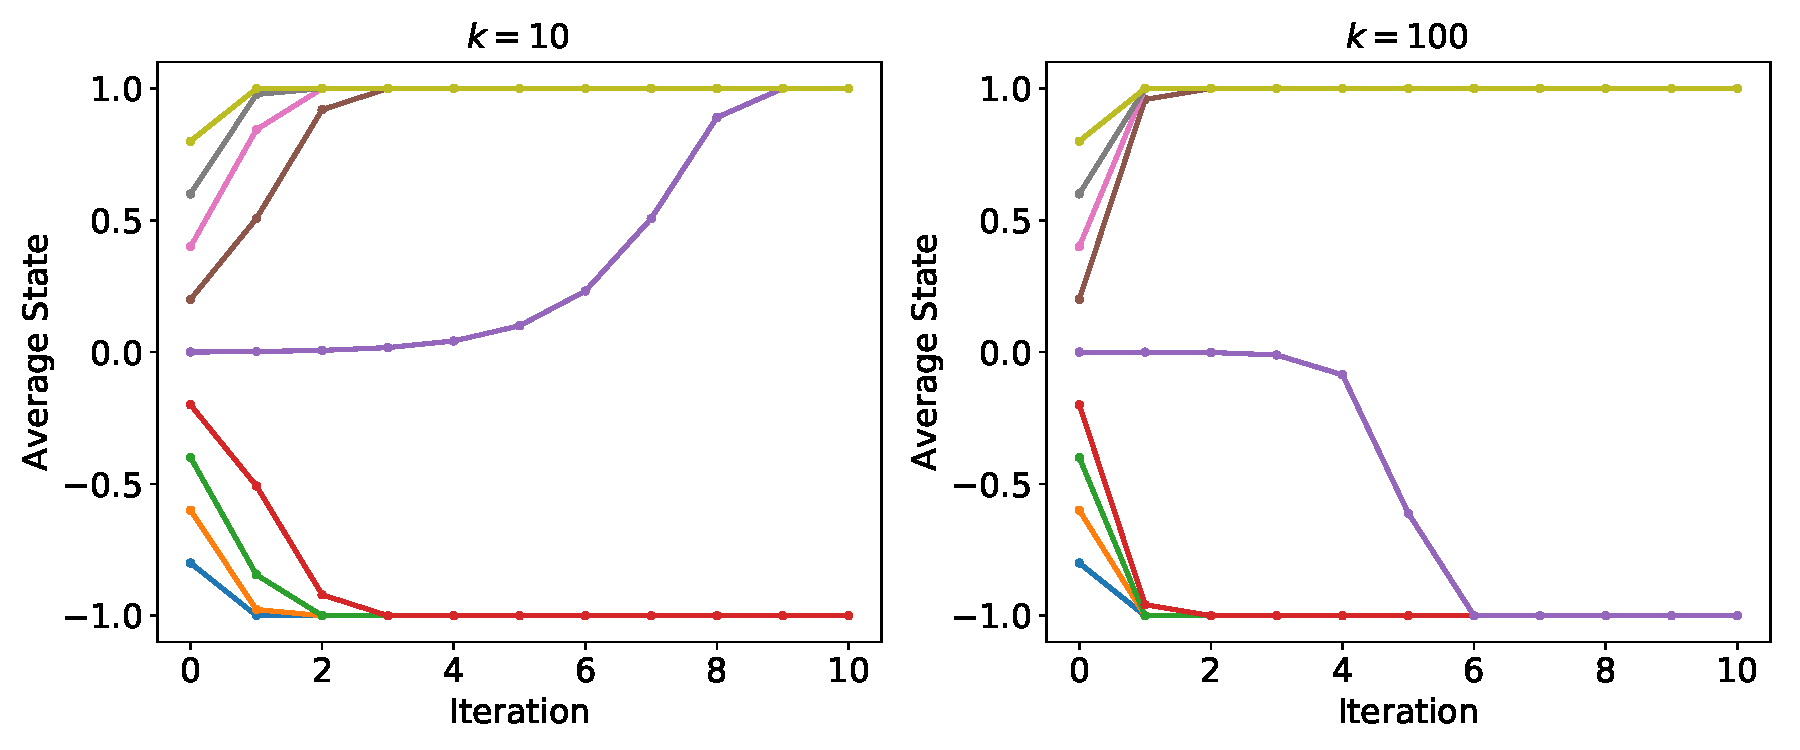
\includegraphics[width=\linewidth]{fig/consensus_convergence}
\caption{Average state of the system converges to either 1 or -1, both representing global consensus. MVCA converges to consensus state which is the state of the majority nodes in just a few steps even with only 10 neighboring nodes in a 1,000,000 nodes network. Increasing the number of neighbors accelerates convergence. Note that when exactly half of the nodes are in one state while the other half in the other state, the converged state could be either one.}
\label{fig:consensus_convergence}
\end{figure*}

To show the performance of our consensus algorithm, we apply it to a simulated network with $N=1,000,000$ nodes. Each node has $k$ neighbors randomly selected from the network. At each iteration, its state is updated based on the states of its $k$ neighbors plus its own state using MVCA rule as proposed above. Neighbors are one directional so that $J$ is not guaranteed to be symmetric. Initially (iteration 0), the state of each node is independently chosen to be 1 or -1 with some probability. The simulation is run for several iterations with different $k$, as shown in Fig.~\ref{fig:consensus_convergence}. One can see that the MVCA converges to global consensus state in just a few steps even with $k = 10$, much faster than the theoretical upper bound $kN$. Note that consensus will be reached even when the initial state contains equal number of 1 and -1 nodes. Larger $k$ leads to faster convergence.

It should be mentioned that when $N$ is large, the topology of the random network will be closer to its “typical” case as the probability to have any specific connectivity decreases exponentially as $N$ increases. Thus, one should look at mean convergence time rather than worst case when (and only when) $N$ is large, as in our simulations.

\begin{figure*}[!htp]
\centering
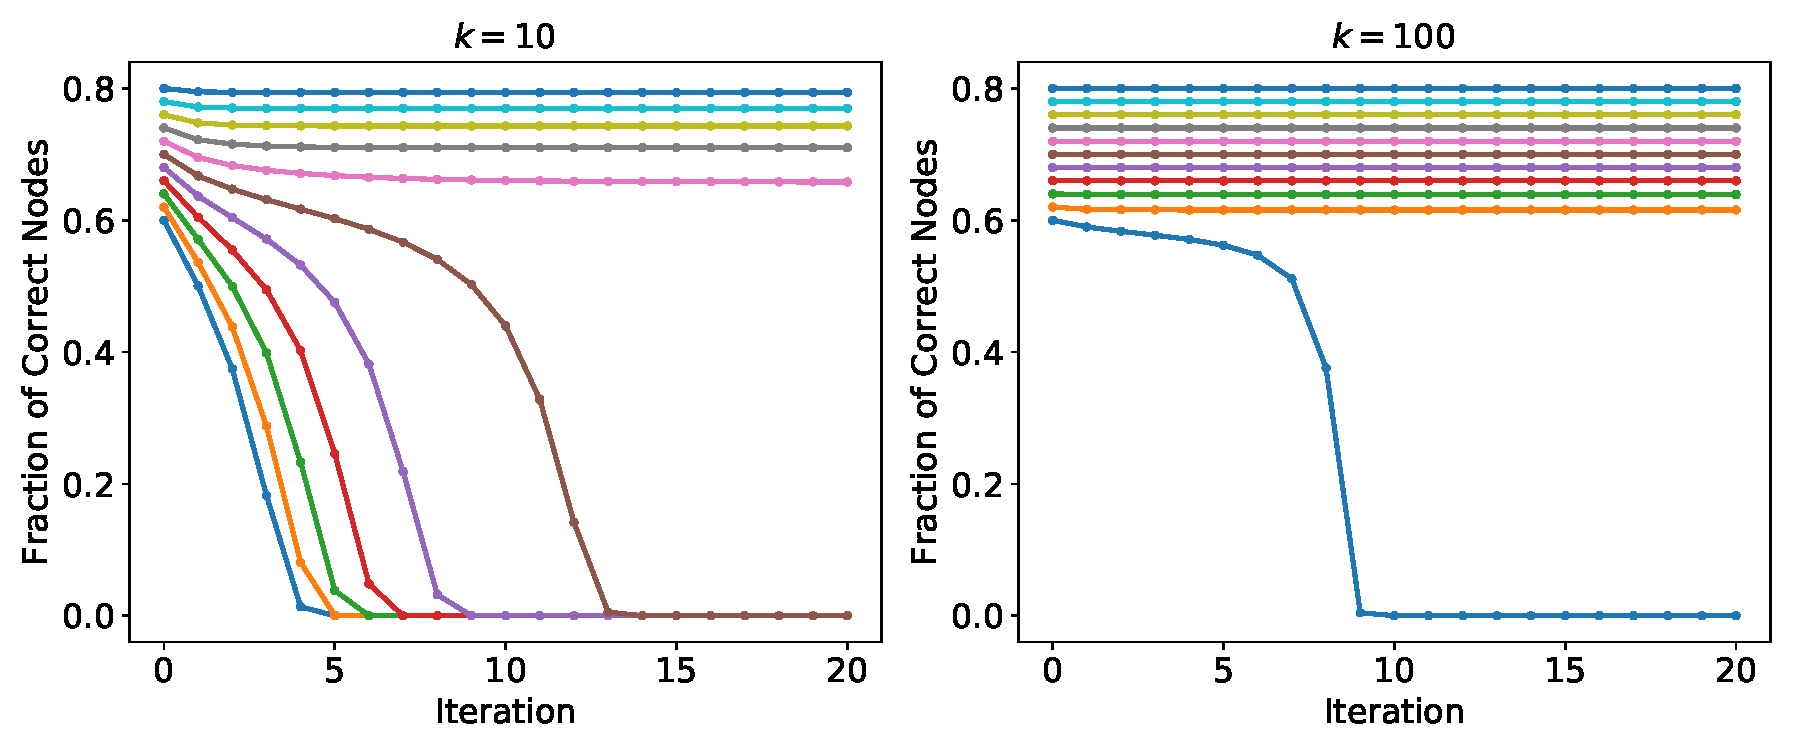
\includegraphics[width=\linewidth]{fig/consensus_malicious}
\caption{Fraction of correct nodes (state 1) under the attack of malicious nodes (state -1) that does not update their states. There is a transition between whether the system will collapse to the wrong state when the initial fraction of malicious nodes changes.}
\label{fig:consensus_malicious}
\end{figure*}

We further simulate the scenario where a fraction of nodes are malicious. In this case “correct” nodes have initial state 1, while malicious nodes have initial state -1 and does not update their states regardless of the states of their neighbors. The goal of the “correct” nodes is to reach consensus on state 1, while the malicious nodes try to reach consensus on state -1. From the results (Fig.~\ref{fig:consensus_malicious}) it can be seen that there is a transition between collapsing to the wrong state (-1) and keeping most correct nodes at the correct state (1). For $N = 1,000,000$ and $k = 10$, the critical fraction of the malicious nodes is around 30\%, which is significant considering the size of $N$. The critical fraction also depends on $k$, as shown in Fig.~\ref{fig:consensus_malicious}. Larger $k$ has two effects: more malicious nodes can be tolerated, and less correct nodes will be affected by malicious nodes.

Results in Fig.~\ref{fig:consensus_convergence} and Fig.~\ref{fig:consensus_malicious} combined show the upper bound and lower bound of the network dynamics with faulty initial states: the former one simulates the case where nodes with incorrect initial state are not malicious, while the latter one simulates the case where nodes with incorrect initial state are all malicious and want the rest of the network to agree on the incorrect state. Network dynamics fall between these two curves with the same initial states whatever strategy faulty nodes (the ones with faulty initial state) take.

\subsubsection{Extension to Asynchronous and Unreliable Networks}

One advantage of using Ising model to describe the system is the natural extension to noisy and unreliable communication channels. The temperature parameter in Ising model controls the amount of noise in the system, and in our case is the randomness in the updating rule. At zero temperature, the updating rule is deterministic, while the rule becomes more random when temperature increases, and eventually becomes purely random when temperature goes to infinity. By including a default state, probabilistic failure of message delivery can be modeled by finite temperature in Ising model. Thus, consensus can still be made as long as noise is under the threshold, as discussed above. The threshold can be computed numerically given the statistics of network connectivity. Asynchronous state update can also be modeled by such noise when communication timeout is added, making it practical for implementation.

\subsection{Proof of Relay}

Consensus in NKN is driven by Proof of Relay (PoR), a useful Proof of Work (PoW) where the expected rewards a node gets depend on its network connectivity and data transmission power. Node proves its relay workload by adding digital signature when forwarding data, which is then accepted by the system through consensus algorithm.

PoR is not a waste of resources since the work performed in PoR benefits the whole network by providing more transmission power. The ``mining'' is redefined as contributing to the data transmission layer, and the only way to get more rewards is providing more transmission power. The competition between nodes in the network will eventually drive the system towards the direction of low latency, high bandwidth data transmission network.

PoR is used for both token mining and transaction verification. On the one hand, token will be rewarded to nodes for data transmission; on the other hand, the expected reward for transaction verification may also depend on PoR, either through election or difficulty adjustment.

For detailed algorithms and economic model, please refer to our separate technical yellow paper \cite{nkn_yellow_paper} and paper on economic model \cite{nkn_economic_model}.

\subsection{Potential Attacks}

Since NKN is designed with attack prevention in mind, it is necessary to review related attack types. Attack analysis and mitigation will be one of the important aspects of NKN development and future work, and will be included in the technical yellow paper \cite{nkn_yellow_paper}.

\begin{enumerate}
\item \textbf{Double spending attack}: double spending attack refers to the case where the same token is spent more than once. In classic blockchain systems, nodes prevent double-spending attack by consensus to confirm the transaction sequence.
\item \textbf{Sybil Attacks}: Sybil attack refers to the case where malicious node pretends to be multiple users. Malicious miners can pretend to deliver more copies and get paid. Physical forwarding is done by creating multiple Sybil identities, but only transmitting data once.
\item \textbf{Denial-of-Service (DoS) Attacks}: an off-line resource centric attack is known as a denial of service attack (DoS). For example, an attacker may want to target a specific account and prevent the account holder from posting transactions.
\item \textbf{Quality-of-Service (QoS) Attacks}: some attackers want to slow down the system performance, potentially reducing the amount of network connectivity and data transfer speed.
\item \textbf{Eclipse attack}: attacker controls the P2P communication network and manipulates a node's neighbors so that it only communicates with malicious nodes. The vulnerability of the network to eclipse attack depends on the peer sampling algorithm, and can be reduced by carefully choosing neighbors.

\item \textbf{Selfish Mining Attacks}: in a selfish mining strategy, the selfish miners maintain two blockchains, one public and one private. Initially, the private blockchain is the same as the public blockchain. The attacker always mine on the private chain, unless the length of the private chain is being caught up by the public chain, in which case the attacker publishes the private chain to get rewards. The attack essentially lower the threshold of 51\% attack as it may be more efficient for other miners to mine the private chain than the public chain. Yet, as an economic attack, selfish mining attack needs to be announced in advance to attract miners.
\item \textbf{Fraud Attacks}: malicious miners can claim large amounts of data to be transmitted but efficiently generate data on-demand using applets. If the applet is smaller than the actual amount of relay data, it increases the likelihood of malicious miners getting block bonus.
\end{enumerate}

\section{Conclusions}

This whitepaper presents a clear and cohesive path towards the construction of NKN system. We consider this work to be a starting point for future research on decentralized network connectivity and data transmission. Future work include, but not limited to, Cellular-Automata-driven routing, Cellular-Automata-based consensus, Proof of Relay etc. NKN has several advantages compared to current platforms.

First, NKN is an ideal networking platform for developing decentralized applications. DApp developers can be completely focused on the creative ideas and innovations that make their products successful for end users, as well as business logic. They no longer need to worry about details of network infrastructure.

Second, NKN incentive model encourages more people to join the network to share and enhance network connectivity and data transmission, changing the entire network structure and creating a huge market. NKN is targeting the trillion-dollar telecommunications business, and aim to provide better connectivity to everyone by incentivize the sharing of unused networking resources, expanding and revolutionize the sharing network.

Compare to current systems, NKN blockchain platform is more suitable for peer-to-peer data transmission and connectivity. In the meantime, this self-incentivized model encourages more nodes to join the network, build a flat network structure, implement multi-path routing, and create a new generation of network transmission structure.

From the perspectives of computing infrastructure innovation, NKN will revolutionize the blockchain ecosystem by blockchainizing the third and probably the last pillar of Internet infrastructure, after Bitcoin and Ethereum blockchainized computing power as well as IPFS and Filecoin blockchainized storage. Complementing the other two pillars of the blockchain revolution, NKN will be the next generation decentralized network that is self-evolving, self-incentivized, and highly scalable. 

NKN is a strategic exploration and innovation of the general network layer infrastructure delivering the next generation network to other fields. A highly reliable, secure and decentralized Internet is essential so that every individual and every industry can achieve their full potential in the digital world. NKN will offer tremendous potential for achieving a fully decentralized peer-to-peer system to make the Internet more efficient, sustainable and secure.

The current network has huge inefficiencies for providing universal connectivity and access for all information and applications. It's time to rebuild the network we really need instead of constantly patching the networks we already own. Let's start building the future Internet, today.

\nocite{*}

\bibliographystyle{unsrt}
\bibliography{whitepaper}

\end{document}
